\documentclass[1p]{elsarticle_modified}
%\bibliographystyle{elsarticle-num}

%\usepackage[colorlinks]{hyperref}
%\usepackage{abbrmath_seonhwa} %\Abb, \Ascr, \Acal ,\Abf, \Afrak
\usepackage{amsfonts}
\usepackage{amssymb}
\usepackage{amsmath}
\usepackage{amsthm}
\usepackage{scalefnt}
\usepackage{amsbsy}
\usepackage{kotex}
\usepackage{caption}
\usepackage{subfig}
\usepackage{color}
\usepackage{graphicx}
\usepackage{xcolor} %% white, black, red, green, blue, cyan, magenta, yellow
\usepackage{float}
\usepackage{setspace}
\usepackage{hyperref}

\usepackage{tikz}
\usetikzlibrary{arrows}

\usepackage{multirow}
\usepackage{array} % fixed length table
\usepackage{hhline}

%%%%%%%%%%%%%%%%%%%%%
\makeatletter
\renewcommand*\env@matrix[1][\arraystretch]{%
	\edef\arraystretch{#1}%
	\hskip -\arraycolsep
	\let\@ifnextchar\new@ifnextchar
	\array{*\c@MaxMatrixCols c}}
\makeatother %https://tex.stackexchange.com/questions/14071/how-can-i-increase-the-line-spacing-in-a-matrix
%%%%%%%%%%%%%%%

\usepackage[normalem]{ulem}

\newcommand{\msout}[1]{\ifmmode\text{\sout{\ensuremath{#1}}}\else\sout{#1}\fi}
%SOURCE: \msout is \stkout macro in https://tex.stackexchange.com/questions/20609/strikeout-in-math-mode

\newcommand{\cancel}[1]{
	\ifmmode
	{\color{red}\msout{#1}}
	\else
	{\color{red}\sout{#1}}
	\fi
}

\newcommand{\add}[1]{
	{\color{blue}\uwave{#1}}
}

\newcommand{\replace}[2]{
	\ifmmode
	{\color{red}\msout{#1}}{\color{blue}\uwave{#2}}
	\else
	{\color{red}\sout{#1}}{\color{blue}\uwave{#2}}
	\fi
}

\newcommand{\Sol}{\mathcal{S}} %segment
\newcommand{\D}{D} %diagram
\newcommand{\A}{\mathcal{A}} %arc


%%%%%%%%%%%%%%%%%%%%%%%%%%%%%5 test

\def\sl{\operatorname{\textup{SL}}(2,\Cbb)}
\def\psl{\operatorname{\textup{PSL}}(2,\Cbb)}
\def\quan{\mkern 1mu \triangleright \mkern 1mu}

\theoremstyle{definition}
\newtheorem{thm}{Theorem}[section]
\newtheorem{prop}[thm]{Proposition}
\newtheorem{lem}[thm]{Lemma}
\newtheorem{ques}[thm]{Question}
\newtheorem{cor}[thm]{Corollary}
\newtheorem{defn}[thm]{Definition}
\newtheorem{exam}[thm]{Example}
\newtheorem{rmk}[thm]{Remark}
\newtheorem{alg}[thm]{Algorithm}

\newcommand{\I}{\sqrt{-1}}
\begin{document}

%\begin{frontmatter}
%
%\title{Boundary parabolic representations of knots up to 8 crossings}
%
%%% Group authors per affiliation:
%\author{Yunhi Cho} 
%\address{Department of Mathematics, University of Seoul, Seoul, Korea}
%\ead{yhcho@uos.ac.kr}
%
%
%\author{Seonhwa Kim} %\fnref{s_kim}}
%\address{Center for Geometry and Physics, Institute for Basic Science, Pohang, 37673, Korea}
%\ead{ryeona17@ibs.re.kr}
%
%\author{Hyuk Kim}
%\address{Department of Mathematical Sciences, Seoul National University, Seoul 08826, Korea}
%\ead{hyukkim@snu.ac.kr}
%
%\author{Seokbeom Yoon}
%\address{Department of Mathematical Sciences, Seoul National University, Seoul, 08826,  Korea}
%\ead{sbyoon15@snu.ac.kr}
%
%\begin{abstract}
%We find all boundary parabolic representation of knots up to 8 crossings.
%
%\end{abstract}
%\begin{keyword}
%    \MSC[2010] 57M25 
%\end{keyword}
%
%\end{frontmatter}

%\linenumbers
%\tableofcontents
%
\newcommand\colored[1]{\textcolor{white}{\rule[-0.35ex]{0.8em}{1.4ex}}\kern-0.8em\color{red} #1}%
%\newcommand\colored[1]{\textcolor{white}{ #1}\kern-2.17ex	\textcolor{white}{ #1}\kern-1.81ex	\textcolor{white}{ #1}\kern-2.15ex\color{red}#1	}

{\Large $\underline{12a_{0325}~(K12a_{0325})}$}

\setlength{\tabcolsep}{10pt}
\renewcommand{\arraystretch}{1.6}
\vspace{1cm}\begin{tabular}{m{100pt}>{\centering\arraybackslash}m{274pt}}
\multirow{5}{120pt}{
	\centering
	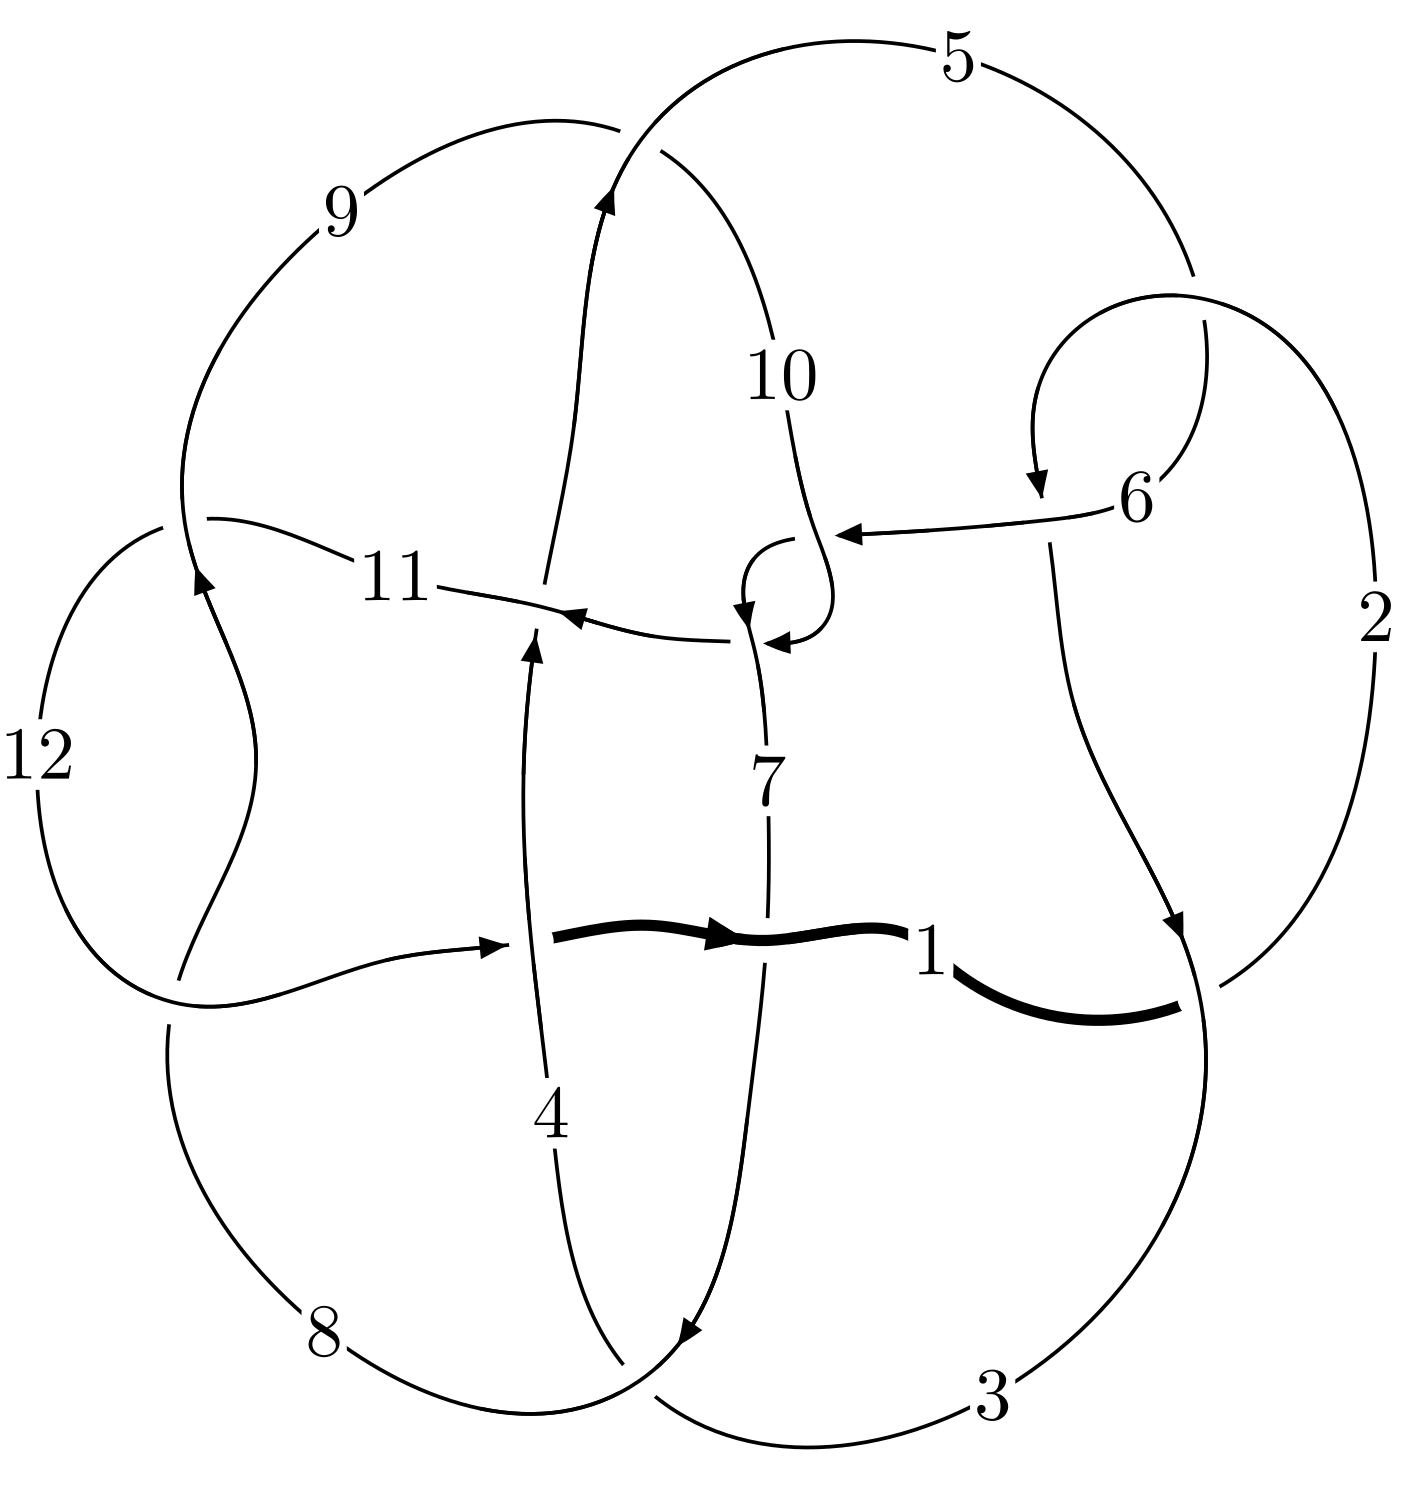
\includegraphics[width=112pt]{../../../GIT/diagram.site/Diagrams/png/1126_12a_0325.png}\\
\ \ \ A knot diagram\footnotemark}&
\allowdisplaybreaks
\textbf{Linearized knot diagam} \\
\cline{2-2}
 &
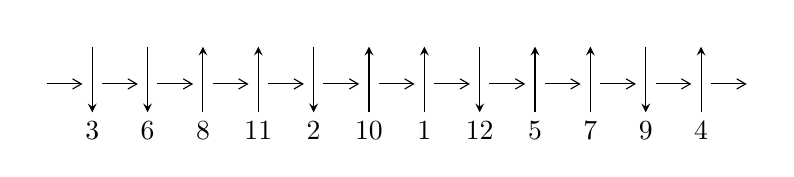
\begin{tikzpicture}[x=20pt, y=17pt]
	% nodes
	\node (C0) at (0, 0) {};
	\node (C1) at (1, 0) {};
	\node (C1U) at (1, +1) {};
	\node (C1D) at (1, -1) {3};

	\node (C2) at (2, 0) {};
	\node (C2U) at (2, +1) {};
	\node (C2D) at (2, -1) {6};

	\node (C3) at (3, 0) {};
	\node (C3U) at (3, +1) {};
	\node (C3D) at (3, -1) {8};

	\node (C4) at (4, 0) {};
	\node (C4U) at (4, +1) {};
	\node (C4D) at (4, -1) {11};

	\node (C5) at (5, 0) {};
	\node (C5U) at (5, +1) {};
	\node (C5D) at (5, -1) {2};

	\node (C6) at (6, 0) {};
	\node (C6U) at (6, +1) {};
	\node (C6D) at (6, -1) {10};

	\node (C7) at (7, 0) {};
	\node (C7U) at (7, +1) {};
	\node (C7D) at (7, -1) {1};

	\node (C8) at (8, 0) {};
	\node (C8U) at (8, +1) {};
	\node (C8D) at (8, -1) {12};

	\node (C9) at (9, 0) {};
	\node (C9U) at (9, +1) {};
	\node (C9D) at (9, -1) {5};

	\node (C10) at (10, 0) {};
	\node (C10U) at (10, +1) {};
	\node (C10D) at (10, -1) {7};

	\node (C11) at (11, 0) {};
	\node (C11U) at (11, +1) {};
	\node (C11D) at (11, -1) {9};

	\node (C12) at (12, 0) {};
	\node (C12U) at (12, +1) {};
	\node (C12D) at (12, -1) {4};
	\node (C13) at (13, 0) {};

	% arrows
	\draw[->,>={angle 60}]
	(C0) edge (C1) (C1) edge (C2) (C2) edge (C3) (C3) edge (C4) (C4) edge (C5) (C5) edge (C6) (C6) edge (C7) (C7) edge (C8) (C8) edge (C9) (C9) edge (C10) (C10) edge (C11) (C11) edge (C12) (C12) edge (C13) ;	\draw[->,>=stealth]
	(C1U) edge (C1D) (C2U) edge (C2D) (C3D) edge (C3U) (C4D) edge (C4U) (C5U) edge (C5D) (C6D) edge (C6U) (C7D) edge (C7U) (C8U) edge (C8D) (C9D) edge (C9U) (C10D) edge (C10U) (C11U) edge (C11D) (C12D) edge (C12U) ;
	\end{tikzpicture} \\
\hhline{~~} \\& 
\textbf{Solving Sequence} \\ \cline{2-2} 
 &
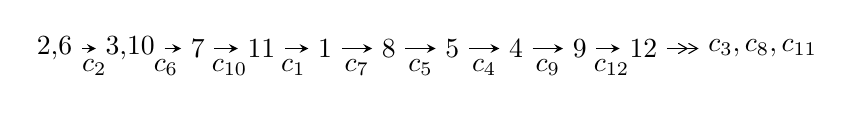
\begin{tikzpicture}[x=23pt, y=7pt]
	% node
	\node (A0) at (-1/8, 0) {2,6};
	\node (A1) at (17/16, 0) {3,10};
	\node (A2) at (17/8, 0) {7};
	\node (A3) at (25/8, 0) {11};
	\node (A4) at (33/8, 0) {1};
	\node (A5) at (41/8, 0) {8};
	\node (A6) at (49/8, 0) {5};
	\node (A7) at (57/8, 0) {4};
	\node (A8) at (65/8, 0) {9};
	\node (A9) at (73/8, 0) {12};
	\node (C1) at (1/2, -1) {$c_{2}$};
	\node (C2) at (13/8, -1) {$c_{6}$};
	\node (C3) at (21/8, -1) {$c_{10}$};
	\node (C4) at (29/8, -1) {$c_{1}$};
	\node (C5) at (37/8, -1) {$c_{7}$};
	\node (C6) at (45/8, -1) {$c_{5}$};
	\node (C7) at (53/8, -1) {$c_{4}$};
	\node (C8) at (61/8, -1) {$c_{9}$};
	\node (C9) at (69/8, -1) {$c_{12}$};
	\node (A10) at (11, 0) {$c_{3},c_{8},c_{11}$};

	% edge
	\draw[->,>=stealth]	
	(A0) edge (A1) (A1) edge (A2) (A2) edge (A3) (A3) edge (A4) (A4) edge (A5) (A5) edge (A6) (A6) edge (A7) (A7) edge (A8) (A8) edge (A9) ;
	\draw[->>,>={angle 60}]	
	(A9) edge (A10);
\end{tikzpicture} \\ 

\end{tabular} \\

\footnotetext{
The image of knot diagram is generated by the software ``\textbf{Draw programme}" developed by Andrew Bartholomew(\url{http://www.layer8.co.uk/maths/draw/index.htm\#Running-draw}), where we modified some parts for our purpose(\url{https://github.com/CATsTAILs/LinksPainter}).
}\phantom \\ \newline 
\centering \textbf{Ideals for irreducible components\footnotemark of $X_{\text{par}}$} 
 
\begin{align*}
I^u_{1}&=\langle 
2.44329\times10^{482} u^{152}-7.61384\times10^{482} u^{151}+\cdots+5.78608\times10^{483} b-1.24996\times10^{485},\\
\phantom{I^u_{1}}&\phantom{= \langle  }-2.64221\times10^{485} u^{152}+9.59872\times10^{485} u^{151}+\cdots+4.66358\times10^{486} a-5.87365\times10^{487},\\
\phantom{I^u_{1}}&\phantom{= \langle  }u^{153}-4 u^{152}+\cdots-1308 u+403\rangle \\
I^u_{2}&=\langle 
-151829464 u^{34}-651172393 u^{33}+\cdots+1552697 b+149127254,\\
\phantom{I^u_{2}}&\phantom{= \langle  }-32108261 u^{34}-103994396 u^{33}+\cdots+1552697 a-12080656,\;u^{35}+5 u^{34}+\cdots-4 u-1\rangle \\
I^u_{3}&=\langle 
b-2 a-1,\;a^2+a+1,\;u+1\rangle \\
I^u_{4}&=\langle 
- a^3 b- a^3+b^2-2 b a+3 a^2+a-2,\;a^4- a^2+1,\;u-1\rangle \\
I^u_{5}&=\langle 
- u^8+2 u^7-2 u^4+b+u,\;- u^8+2 u^7+u^6-2 u^5-3 u^4+2 u^3+2 u^2+a-1,\\
\phantom{I^u_{5}}&\phantom{= \langle  }u^9-2 u^8- u^7+2 u^6+3 u^5-2 u^4-2 u^3+u+1\rangle \\
\\
\end{align*}
\raggedright * 5 irreducible components of $\dim_{\mathbb{C}}=0$, with total 207 representations.\\
\footnotetext{All coefficients of polynomials are rational numbers. But the coefficients are sometimes approximated in decimal forms when there is not enough margin.}
\newpage
\renewcommand{\arraystretch}{1}
\centering \section*{I. $I^u_{1}= \langle 2.44\times10^{482} u^{152}-7.61\times10^{482} u^{151}+\cdots+5.79\times10^{483} b-1.25\times10^{485},\;-2.64\times10^{485} u^{152}+9.60\times10^{485} u^{151}+\cdots+4.66\times10^{486} a-5.87\times10^{487},\;u^{153}-4 u^{152}+\cdots-1308 u+403 \rangle$}
\flushleft \textbf{(i) Arc colorings}\\
\begin{tabular}{m{7pt} m{180pt} m{7pt} m{180pt} }
\flushright $a_{2}=$&$\begin{pmatrix}1\\0\end{pmatrix}$ \\
\flushright $a_{6}=$&$\begin{pmatrix}0\\u\end{pmatrix}$ \\
\flushright $a_{3}=$&$\begin{pmatrix}1\\u^2\end{pmatrix}$ \\
\flushright $a_{10}=$&$\begin{pmatrix}0.0566562 u^{152}-0.205823 u^{151}+\cdots-38.0727 u+12.5947\\-0.0422271 u^{152}+0.131589 u^{151}+\cdots-54.6888 u+21.6029\end{pmatrix}$ \\
\flushright $a_{7}=$&$\begin{pmatrix}0.00265909 u^{152}-0.00685318 u^{151}+\cdots-17.1575 u+4.86894\\0.00422906 u^{152}+0.00397335 u^{151}+\cdots+9.07092 u-3.66335\end{pmatrix}$ \\
\flushright $a_{11}=$&$\begin{pmatrix}-0.0405739 u^{152}+0.158089 u^{151}+\cdots+92.2622 u-8.25737\\-0.0194224 u^{152}+0.0553301 u^{151}+\cdots+12.8460 u-10.3832\end{pmatrix}$ \\
\flushright $a_{1}=$&$\begin{pmatrix}- u^2+1\\- u^4\end{pmatrix}$ \\
\flushright $a_{8}=$&$\begin{pmatrix}-0.0307886 u^{152}+0.0997291 u^{151}+\cdots-40.0301 u+9.22919\\-0.0327039 u^{152}+0.116997 u^{151}+\cdots-26.8406 u+10.0730\end{pmatrix}$ \\
\flushright $a_{5}=$&$\begin{pmatrix}u\\u\end{pmatrix}$ \\
\flushright $a_{4}=$&$\begin{pmatrix}-0.0341103 u^{152}+0.146828 u^{151}+\cdots+72.8214 u+10.7106\\-0.0262821 u^{152}+0.106569 u^{151}+\cdots-17.8242 u+20.3022\end{pmatrix}$ \\
\flushright $a_{9}=$&$\begin{pmatrix}0.107309 u^{152}-0.383646 u^{151}+\cdots-1.89981 u-10.8282\\0.00842534 u^{152}-0.0462346 u^{151}+\cdots-18.5159 u-1.82006\end{pmatrix}$ \\
\flushright $a_{12}=$&$\begin{pmatrix}-0.00158834 u^{152}+0.0137909 u^{151}+\cdots+82.2526 u-20.2425\\0.0437817 u^{152}-0.135616 u^{151}+\cdots+54.3146 u-23.0555\end{pmatrix}$\\&\end{tabular}
\flushleft \textbf{(ii) Obstruction class $= -1$}\\~\\
\flushleft \textbf{(iii) Cusp Shapes $= 0.179165 u^{152}-0.633170 u^{151}+\cdots+417.974 u-142.860$}\\~\\
\newpage\renewcommand{\arraystretch}{1}
\flushleft \textbf{(iv) u-Polynomials at the component}\newline \\
\begin{tabular}{m{50pt}|m{274pt}}
Crossings & \hspace{64pt}u-Polynomials at each crossing \\
\hline $$\begin{aligned}c_{1}\end{aligned}$$&$\begin{aligned}
&u^{153}+56 u^{152}+\cdots+5203262 u+162409
\end{aligned}$\\
\hline $$\begin{aligned}c_{2},c_{5}\end{aligned}$$&$\begin{aligned}
&u^{153}+4 u^{152}+\cdots-1308 u-403
\end{aligned}$\\
\hline $$\begin{aligned}c_{3}\end{aligned}$$&$\begin{aligned}
&u^{153}+4 u^{152}+\cdots+3298135 u+149921
\end{aligned}$\\
\hline $$\begin{aligned}c_{4}\end{aligned}$$&$\begin{aligned}
&u^{153}+2 u^{152}+\cdots-590459 u+127561
\end{aligned}$\\
\hline $$\begin{aligned}c_{6},c_{10}\end{aligned}$$&$\begin{aligned}
&u^{153}+4 u^{152}+\cdots-32672 u-1744
\end{aligned}$\\
\hline $$\begin{aligned}c_{7}\end{aligned}$$&$\begin{aligned}
&u^{153}-4 u^{152}+\cdots-54959 u-3812
\end{aligned}$\\
\hline $$\begin{aligned}c_{8},c_{11}\end{aligned}$$&$\begin{aligned}
&u^{153}-11 u^{152}+\cdots+444 u-9
\end{aligned}$\\
\hline $$\begin{aligned}c_{9}\end{aligned}$$&$\begin{aligned}
&u^{153}-36 u^{151}+\cdots-415921821 u-28550563
\end{aligned}$\\
\hline $$\begin{aligned}c_{12}\end{aligned}$$&$\begin{aligned}
&u^{153}+12 u^{152}+\cdots-183 u+11
\end{aligned}$\\
\hline
\end{tabular}\\~\\
\newpage\renewcommand{\arraystretch}{1}
\flushleft \textbf{(v) Riley Polynomials at the component}\newline \\
\begin{tabular}{m{50pt}|m{274pt}}
Crossings & \hspace{64pt}Riley Polynomials at each crossing \\
\hline $$\begin{aligned}c_{1}\end{aligned}$$&$\begin{aligned}
&y^{153}+88 y^{152}+\cdots+4445192262174 y-26376683281
\end{aligned}$\\
\hline $$\begin{aligned}c_{2},c_{5}\end{aligned}$$&$\begin{aligned}
&y^{153}-56 y^{152}+\cdots+5203262 y-162409
\end{aligned}$\\
\hline $$\begin{aligned}c_{3}\end{aligned}$$&$\begin{aligned}
&y^{153}-58 y^{152}+\cdots+6128533920791 y-22476306241
\end{aligned}$\\
\hline $$\begin{aligned}c_{4}\end{aligned}$$&$\begin{aligned}
&y^{153}-22 y^{152}+\cdots+398065340131 y-16271808721
\end{aligned}$\\
\hline $$\begin{aligned}c_{6},c_{10}\end{aligned}$$&$\begin{aligned}
&y^{153}-96 y^{152}+\cdots+45684864 y-3041536
\end{aligned}$\\
\hline $$\begin{aligned}c_{7}\end{aligned}$$&$\begin{aligned}
&y^{153}-4 y^{152}+\cdots+642535585 y-14531344
\end{aligned}$\\
\hline $$\begin{aligned}c_{8},c_{11}\end{aligned}$$&$\begin{aligned}
&y^{153}+127 y^{152}+\cdots+10368 y-81
\end{aligned}$\\
\hline $$\begin{aligned}c_{9}\end{aligned}$$&$\begin{aligned}
&y^{153}-72 y^{152}+\cdots+144574949507127535 y-815134647616969
\end{aligned}$\\
\hline $$\begin{aligned}c_{12}\end{aligned}$$&$\begin{aligned}
&y^{153}-16 y^{152}+\cdots+16637 y-121
\end{aligned}$\\
\hline
\end{tabular}\\~\\
\newpage\flushleft \textbf{(vi) Complex Volumes and Cusp Shapes}
$$\begin{array}{c|c|c}  
\text{Solutions to }I^u_{1}& \I (\text{vol} + \sqrt{-1}CS) & \text{Cusp shape}\\
 \hline 
\begin{aligned}
u &= -0.675420 + 0.737717 I \\
a &= \phantom{-}1.31203 + 0.65867 I \\
b &= \phantom{-}0.192324 - 0.026203 I\end{aligned}
 & \phantom{-}3.56258 - 1.68630 I & \phantom{-0.000000 } 0 \\ \hline\begin{aligned}
u &= -0.675420 - 0.737717 I \\
a &= \phantom{-}1.31203 - 0.65867 I \\
b &= \phantom{-}0.192324 + 0.026203 I\end{aligned}
 & \phantom{-}3.56258 + 1.68630 I & \phantom{-0.000000 } 0 \\ \hline\begin{aligned}
u &= \phantom{-}0.712633 + 0.692997 I \\
a &= -0.853056 - 0.873264 I \\
b &= -0.267587 - 1.229830 I\end{aligned}
 & -0.06386 + 2.09461 I & \phantom{-0.000000 } 0 \\ \hline\begin{aligned}
u &= \phantom{-}0.712633 - 0.692997 I \\
a &= -0.853056 + 0.873264 I \\
b &= -0.267587 + 1.229830 I\end{aligned}
 & -0.06386 - 2.09461 I & \phantom{-0.000000 } 0 \\ \hline\begin{aligned}
u &= \phantom{-}0.833577 + 0.529608 I \\
a &= -0.808363 + 0.906087 I \\
b &= \phantom{-}0.30919 + 1.83699 I\end{aligned}
 & \phantom{-}1.92792 - 4.14574 I & \phantom{-0.000000 } 0 \\ \hline\begin{aligned}
u &= \phantom{-}0.833577 - 0.529608 I \\
a &= -0.808363 - 0.906087 I \\
b &= \phantom{-}0.30919 - 1.83699 I\end{aligned}
 & \phantom{-}1.92792 + 4.14574 I & \phantom{-0.000000 } 0 \\ \hline\begin{aligned}
u &= \phantom{-}0.726189 + 0.712147 I \\
a &= \phantom{-}1.234100 - 0.684681 I \\
b &= -0.500158 + 0.082418 I\end{aligned}
 & \phantom{-}9.74457 + 4.78074 I & \phantom{-0.000000 } 0 \\ \hline\begin{aligned}
u &= \phantom{-}0.726189 - 0.712147 I \\
a &= \phantom{-}1.234100 + 0.684681 I \\
b &= -0.500158 - 0.082418 I\end{aligned}
 & \phantom{-}9.74457 - 4.78074 I & \phantom{-0.000000 } 0 \\ \hline\begin{aligned}
u &= -0.848864 + 0.565331 I \\
a &= \phantom{-}1.117470 - 0.856923 I \\
b &= \phantom{-}0.43012 - 1.41259 I\end{aligned}
 & -0.424170 - 0.231230 I & \phantom{-0.000000 } 0 \\ \hline\begin{aligned}
u &= -0.848864 - 0.565331 I \\
a &= \phantom{-}1.117470 + 0.856923 I \\
b &= \phantom{-}0.43012 + 1.41259 I\end{aligned}
 & -0.424170 + 0.231230 I & \phantom{-0.000000 } 0\\
 \hline 
 \end{array}$$\newpage$$\begin{array}{c|c|c}  
\text{Solutions to }I^u_{1}& \I (\text{vol} + \sqrt{-1}CS) & \text{Cusp shape}\\
 \hline 
\begin{aligned}
u &= \phantom{-}0.637354 + 0.807506 I \\
a &= \phantom{-}0.866602 + 0.671451 I \\
b &= -0.126080 + 1.155340 I\end{aligned}
 & \phantom{-}5.44000 + 7.90600 I & \phantom{-0.000000 } 0 \\ \hline\begin{aligned}
u &= \phantom{-}0.637354 - 0.807506 I \\
a &= \phantom{-}0.866602 - 0.671451 I \\
b &= -0.126080 - 1.155340 I\end{aligned}
 & \phantom{-}5.44000 - 7.90600 I & \phantom{-0.000000 } 0 \\ \hline\begin{aligned}
u &= -0.750041 + 0.616302 I \\
a &= -1.241710 + 0.108581 I \\
b &= -0.256077 + 1.381250 I\end{aligned}
 & \phantom{-}2.67326 - 0.74208 I & \phantom{-0.000000 } 0 \\ \hline\begin{aligned}
u &= -0.750041 - 0.616302 I \\
a &= -1.241710 - 0.108581 I \\
b &= -0.256077 - 1.381250 I\end{aligned}
 & \phantom{-}2.67326 + 0.74208 I & \phantom{-0.000000 } 0 \\ \hline\begin{aligned}
u &= -0.658054 + 0.804069 I \\
a &= -0.608800 + 0.419900 I \\
b &= \phantom{-}0.433604 + 0.871465 I\end{aligned}
 & \phantom{-}6.01531 + 0.24800 I & \phantom{-0.000000 } 0 \\ \hline\begin{aligned}
u &= -0.658054 - 0.804069 I \\
a &= -0.608800 - 0.419900 I \\
b &= \phantom{-}0.433604 - 0.871465 I\end{aligned}
 & \phantom{-}6.01531 - 0.24800 I & \phantom{-0.000000 } 0 \\ \hline\begin{aligned}
u &= \phantom{-}0.797105 + 0.686679 I \\
a &= -1.26136 + 0.71763 I \\
b &= \phantom{-}0.022369 + 0.437942 I\end{aligned}
 & \phantom{-}5.44169 - 1.59304 I & \phantom{-0.000000 } 0 \\ \hline\begin{aligned}
u &= \phantom{-}0.797105 - 0.686679 I \\
a &= -1.26136 - 0.71763 I \\
b &= \phantom{-}0.022369 - 0.437942 I\end{aligned}
 & \phantom{-}5.44169 + 1.59304 I & \phantom{-0.000000 } 0 \\ \hline\begin{aligned}
u &= -0.911731 + 0.552948 I \\
a &= -0.477581 + 1.096580 I \\
b &= \phantom{-}0.07984 + 1.80339 I\end{aligned}
 & -0.60988 + 4.66390 I & \phantom{-0.000000 } 0 \\ \hline\begin{aligned}
u &= -0.911731 - 0.552948 I \\
a &= -0.477581 - 1.096580 I \\
b &= \phantom{-}0.07984 - 1.80339 I\end{aligned}
 & -0.60988 - 4.66390 I & \phantom{-0.000000 } 0\\
 \hline 
 \end{array}$$\newpage$$\begin{array}{c|c|c}  
\text{Solutions to }I^u_{1}& \I (\text{vol} + \sqrt{-1}CS) & \text{Cusp shape}\\
 \hline 
\begin{aligned}
u &= \phantom{-}1.044140 + 0.221555 I \\
a &= \phantom{-}0.234186 + 0.137129 I \\
b &= \phantom{-}0.900973 - 0.502033 I\end{aligned}
 & -0.419188 + 0.000601 I & \phantom{-0.000000 } 0 \\ \hline\begin{aligned}
u &= \phantom{-}1.044140 - 0.221555 I \\
a &= \phantom{-}0.234186 - 0.137129 I \\
b &= \phantom{-}0.900973 + 0.502033 I\end{aligned}
 & -0.419188 - 0.000601 I & \phantom{-0.000000 } 0 \\ \hline\begin{aligned}
u &= \phantom{-}0.223508 + 0.900376 I \\
a &= \phantom{-}0.048702 - 1.141970 I \\
b &= -0.098374 - 0.290094 I\end{aligned}
 & \phantom{-}1.69039 - 3.74324 I & \phantom{-0.000000 } 0 \\ \hline\begin{aligned}
u &= \phantom{-}0.223508 - 0.900376 I \\
a &= \phantom{-}0.048702 + 1.141970 I \\
b &= -0.098374 + 0.290094 I\end{aligned}
 & \phantom{-}1.69039 + 3.74324 I & \phantom{-0.000000 } 0 \\ \hline\begin{aligned}
u &= \phantom{-}1.046970 + 0.275240 I \\
a &= -0.612920 + 0.491990 I \\
b &= -1.94412 + 0.94083 I\end{aligned}
 & -2.13134 - 2.48634 I & \phantom{-0.000000 } 0 \\ \hline\begin{aligned}
u &= \phantom{-}1.046970 - 0.275240 I \\
a &= -0.612920 - 0.491990 I \\
b &= -1.94412 - 0.94083 I\end{aligned}
 & -2.13134 + 2.48634 I & \phantom{-0.000000 } 0 \\ \hline\begin{aligned}
u &= \phantom{-}0.855023 + 0.329474 I \\
a &= -0.44008 + 1.38498 I \\
b &= \phantom{-}0.14747 + 1.64774 I\end{aligned}
 & -1.65566 - 4.20561 I & \phantom{-0.000000 } 0 \\ \hline\begin{aligned}
u &= \phantom{-}0.855023 - 0.329474 I \\
a &= -0.44008 - 1.38498 I \\
b &= \phantom{-}0.14747 - 1.64774 I\end{aligned}
 & -1.65566 + 4.20561 I & \phantom{-0.000000 } 0 \\ \hline\begin{aligned}
u &= -0.908445 + 0.098730 I \\
a &= -1.211430 - 0.055199 I \\
b &= -2.53684 + 0.64359 I\end{aligned}
 & \phantom{-}5.43502 - 5.17729 I & \phantom{-0.000000 } 0 \\ \hline\begin{aligned}
u &= -0.908445 - 0.098730 I \\
a &= -1.211430 + 0.055199 I \\
b &= -2.53684 - 0.64359 I\end{aligned}
 & \phantom{-}5.43502 + 5.17729 I & \phantom{-0.000000 } 0\\
 \hline 
 \end{array}$$\newpage$$\begin{array}{c|c|c}  
\text{Solutions to }I^u_{1}& \I (\text{vol} + \sqrt{-1}CS) & \text{Cusp shape}\\
 \hline 
\begin{aligned}
u &= \phantom{-}1.042560 + 0.314422 I \\
a &= \phantom{-}0.005034 - 0.658412 I \\
b &= -0.629969 - 1.128490 I\end{aligned}
 & -1.84749 - 0.93407 I & \phantom{-0.000000 } 0 \\ \hline\begin{aligned}
u &= \phantom{-}1.042560 - 0.314422 I \\
a &= \phantom{-}0.005034 + 0.658412 I \\
b &= -0.629969 + 1.128490 I\end{aligned}
 & -1.84749 + 0.93407 I & \phantom{-0.000000 } 0 \\ \hline\begin{aligned}
u &= \phantom{-}0.771627 + 0.775380 I \\
a &= \phantom{-}0.299982 + 0.523125 I \\
b &= \phantom{-}0.14897 + 1.55115 I\end{aligned}
 & \phantom{-}4.97087 - 5.83091 I & \phantom{-0.000000 } 0 \\ \hline\begin{aligned}
u &= \phantom{-}0.771627 - 0.775380 I \\
a &= \phantom{-}0.299982 - 0.523125 I \\
b &= \phantom{-}0.14897 - 1.55115 I\end{aligned}
 & \phantom{-}4.97087 + 5.83091 I & \phantom{-0.000000 } 0 \\ \hline\begin{aligned}
u &= \phantom{-}0.891588 + 0.126622 I \\
a &= -1.008690 - 0.627616 I \\
b &= -1.53323 - 0.42808 I\end{aligned}
 & -1.37826 + 1.95591 I & \phantom{-0.000000 } 0 \\ \hline\begin{aligned}
u &= \phantom{-}0.891588 - 0.126622 I \\
a &= -1.008690 + 0.627616 I \\
b &= -1.53323 + 0.42808 I\end{aligned}
 & -1.37826 - 1.95591 I & \phantom{-0.000000 } 0 \\ \hline\begin{aligned}
u &= \phantom{-}0.870067 + 0.203606 I \\
a &= -1.137610 - 0.247333 I \\
b &= \phantom{-}0.18143 - 1.88250 I\end{aligned}
 & -1.52748 + 1.01810 I & \phantom{-0.000000 } 0 \\ \hline\begin{aligned}
u &= \phantom{-}0.870067 - 0.203606 I \\
a &= -1.137610 + 0.247333 I \\
b &= \phantom{-}0.18143 + 1.88250 I\end{aligned}
 & -1.52748 - 1.01810 I & \phantom{-0.000000 } 0 \\ \hline\begin{aligned}
u &= \phantom{-}1.060790 + 0.318839 I \\
a &= \phantom{-}0.250423 - 0.244541 I \\
b &= -0.060557 - 0.528126 I\end{aligned}
 & -1.90791 - 1.30264 I & \phantom{-0.000000 } 0 \\ \hline\begin{aligned}
u &= \phantom{-}1.060790 - 0.318839 I \\
a &= \phantom{-}0.250423 + 0.244541 I \\
b &= -0.060557 + 0.528126 I\end{aligned}
 & -1.90791 + 1.30264 I & \phantom{-0.000000 } 0\\
 \hline 
 \end{array}$$\newpage$$\begin{array}{c|c|c}  
\text{Solutions to }I^u_{1}& \I (\text{vol} + \sqrt{-1}CS) & \text{Cusp shape}\\
 \hline 
\begin{aligned}
u &= \phantom{-}0.850090 + 0.712175 I \\
a &= \phantom{-}1.32657 - 0.67283 I \\
b &= \phantom{-}0.424380 - 0.107176 I\end{aligned}
 & \phantom{-}10.17410 - 7.33774 I & \phantom{-0.000000 } 0 \\ \hline\begin{aligned}
u &= \phantom{-}0.850090 - 0.712175 I \\
a &= \phantom{-}1.32657 + 0.67283 I \\
b &= \phantom{-}0.424380 + 0.107176 I\end{aligned}
 & \phantom{-}10.17410 + 7.33774 I & \phantom{-0.000000 } 0 \\ \hline\begin{aligned}
u &= -0.432157 + 0.775321 I \\
a &= -1.20345 - 1.22917 I \\
b &= -0.025196 - 0.180087 I\end{aligned}
 & \phantom{-}6.52645 - 5.80569 I & \phantom{-0.000000 } 0 \\ \hline\begin{aligned}
u &= -0.432157 - 0.775321 I \\
a &= -1.20345 + 1.22917 I \\
b &= -0.025196 + 0.180087 I\end{aligned}
 & \phantom{-}6.52645 + 5.80569 I & \phantom{-0.000000 } 0 \\ \hline\begin{aligned}
u &= -0.626201 + 0.625096 I \\
a &= -0.838410 - 0.678997 I \\
b &= \phantom{-}1.01490 - 1.77224 I\end{aligned}
 & \phantom{-}4.32590 - 5.42619 I & \phantom{-0.000000 } 0 \\ \hline\begin{aligned}
u &= -0.626201 - 0.625096 I \\
a &= -0.838410 + 0.678997 I \\
b &= \phantom{-}1.01490 + 1.77224 I\end{aligned}
 & \phantom{-}4.32590 + 5.42619 I & \phantom{-0.000000 } 0 \\ \hline\begin{aligned}
u &= -0.570543 + 0.959668 I \\
a &= -0.800270 - 0.848486 I \\
b &= \phantom{-}0.200774 - 0.268302 I\end{aligned}
 & \phantom{-}6.27187 - 2.95983 I & \phantom{-0.000000 } 0 \\ \hline\begin{aligned}
u &= -0.570543 - 0.959668 I \\
a &= -0.800270 + 0.848486 I \\
b &= \phantom{-}0.200774 + 0.268302 I\end{aligned}
 & \phantom{-}6.27187 + 2.95983 I & \phantom{-0.000000 } 0 \\ \hline\begin{aligned}
u &= -1.113800 + 0.077620 I \\
a &= \phantom{-}0.446702 - 0.639826 I \\
b &= -0.32574 - 1.61736 I\end{aligned}
 & -0.77901 + 7.21951 I & \phantom{-0.000000 } 0 \\ \hline\begin{aligned}
u &= -1.113800 - 0.077620 I \\
a &= \phantom{-}0.446702 + 0.639826 I \\
b &= -0.32574 + 1.61736 I\end{aligned}
 & -0.77901 - 7.21951 I & \phantom{-0.000000 } 0\\
 \hline 
 \end{array}$$\newpage$$\begin{array}{c|c|c}  
\text{Solutions to }I^u_{1}& \I (\text{vol} + \sqrt{-1}CS) & \text{Cusp shape}\\
 \hline 
\begin{aligned}
u &= \phantom{-}0.657255 + 0.909275 I \\
a &= \phantom{-}1.088970 - 0.712066 I \\
b &= -0.123532 - 0.187303 I\end{aligned}
 & \phantom{-}4.36186 + 7.97183 I & \phantom{-0.000000 } 0 \\ \hline\begin{aligned}
u &= \phantom{-}0.657255 - 0.909275 I \\
a &= \phantom{-}1.088970 + 0.712066 I \\
b &= -0.123532 + 0.187303 I\end{aligned}
 & \phantom{-}4.36186 - 7.97183 I & \phantom{-0.000000 } 0 \\ \hline\begin{aligned}
u &= -0.914797 + 0.660919 I \\
a &= \phantom{-}0.739234 + 0.676124 I \\
b &= -0.83643 + 1.47876 I\end{aligned}
 & \phantom{-}1.29894 + 5.17544 I & \phantom{-0.000000 } 0 \\ \hline\begin{aligned}
u &= -0.914797 - 0.660919 I \\
a &= \phantom{-}0.739234 - 0.676124 I \\
b &= -0.83643 - 1.47876 I\end{aligned}
 & \phantom{-}1.29894 - 5.17544 I & \phantom{-0.000000 } 0 \\ \hline\begin{aligned}
u &= -0.760740 + 0.416967 I \\
a &= \phantom{-}1.241350 - 0.136865 I \\
b &= \phantom{-}0.608290 - 1.115850 I\end{aligned}
 & \phantom{-}1.246610 - 0.582741 I & \phantom{-0.000000 } 0 \\ \hline\begin{aligned}
u &= -0.760740 - 0.416967 I \\
a &= \phantom{-}1.241350 + 0.136865 I \\
b &= \phantom{-}0.608290 + 1.115850 I\end{aligned}
 & \phantom{-}1.246610 + 0.582741 I & \phantom{-0.000000 } 0 \\ \hline\begin{aligned}
u &= \phantom{-}0.874822 + 0.719721 I \\
a &= \phantom{-}0.716781 - 1.155820 I \\
b &= \phantom{-}1.23055 - 1.78049 I\end{aligned}
 & \phantom{-}10.10190 + 1.87017 I & \phantom{-0.000000 } 0 \\ \hline\begin{aligned}
u &= \phantom{-}0.874822 - 0.719721 I \\
a &= \phantom{-}0.716781 + 1.155820 I \\
b &= \phantom{-}1.23055 + 1.78049 I\end{aligned}
 & \phantom{-}10.10190 - 1.87017 I & \phantom{-0.000000 } 0 \\ \hline\begin{aligned}
u &= \phantom{-}0.913453 + 0.670384 I \\
a &= -0.777747 + 1.015990 I \\
b &= -1.04270 + 2.14454 I\end{aligned}
 & \phantom{-}5.08027 - 3.64584 I & \phantom{-0.000000 } 0 \\ \hline\begin{aligned}
u &= \phantom{-}0.913453 - 0.670384 I \\
a &= -0.777747 - 1.015990 I \\
b &= -1.04270 - 2.14454 I\end{aligned}
 & \phantom{-}5.08027 + 3.64584 I & \phantom{-0.000000 } 0\\
 \hline 
 \end{array}$$\newpage$$\begin{array}{c|c|c}  
\text{Solutions to }I^u_{1}& \I (\text{vol} + \sqrt{-1}CS) & \text{Cusp shape}\\
 \hline 
\begin{aligned}
u &= -0.959519 + 0.620623 I \\
a &= -0.010563 - 0.987263 I \\
b &= -1.10142 - 1.57540 I\end{aligned}
 & \phantom{-}1.99753 + 5.62196 I & \phantom{-0.000000 } 0 \\ \hline\begin{aligned}
u &= -0.959519 - 0.620623 I \\
a &= -0.010563 + 0.987263 I \\
b &= -1.10142 + 1.57540 I\end{aligned}
 & \phantom{-}1.99753 - 5.62196 I & \phantom{-0.000000 } 0 \\ \hline\begin{aligned}
u &= -0.997511 + 0.567853 I \\
a &= -0.106511 + 0.731704 I \\
b &= \phantom{-}0.52936 + 1.36991 I\end{aligned}
 & \phantom{-}0.03637 + 4.78899 I & \phantom{-0.000000 } 0 \\ \hline\begin{aligned}
u &= -0.997511 - 0.567853 I \\
a &= -0.106511 - 0.731704 I \\
b &= \phantom{-}0.52936 - 1.36991 I\end{aligned}
 & \phantom{-}0.03637 - 4.78899 I & \phantom{-0.000000 } 0 \\ \hline\begin{aligned}
u &= -0.753439 + 0.893258 I \\
a &= -0.685128 - 0.757617 I \\
b &= \phantom{-}0.190907 - 0.138520 I\end{aligned}
 & \phantom{-}8.96953 + 2.45341 I & \phantom{-0.000000 } 0 \\ \hline\begin{aligned}
u &= -0.753439 - 0.893258 I \\
a &= -0.685128 + 0.757617 I \\
b &= \phantom{-}0.190907 + 0.138520 I\end{aligned}
 & \phantom{-}8.96953 - 2.45341 I & \phantom{-0.000000 } 0 \\ \hline\begin{aligned}
u &= \phantom{-}0.921136 + 0.724216 I \\
a &= -0.687688 - 0.470788 I \\
b &= \phantom{-}0.132010 - 0.733189 I\end{aligned}
 & \phantom{-}4.54242 + 0.18184 I & \phantom{-0.000000 } 0 \\ \hline\begin{aligned}
u &= \phantom{-}0.921136 - 0.724216 I \\
a &= -0.687688 + 0.470788 I \\
b &= \phantom{-}0.132010 + 0.733189 I\end{aligned}
 & \phantom{-}4.54242 - 0.18184 I & \phantom{-0.000000 } 0 \\ \hline\begin{aligned}
u &= -0.771547 + 0.297595 I \\
a &= \phantom{-}0.096710 + 1.336130 I \\
b &= \phantom{-}0.27809 + 1.99610 I\end{aligned}
 & -0.90498 + 4.15963 I & \phantom{-0.000000 } 0 \\ \hline\begin{aligned}
u &= -0.771547 - 0.297595 I \\
a &= \phantom{-}0.096710 - 1.336130 I \\
b &= \phantom{-}0.27809 - 1.99610 I\end{aligned}
 & -0.90498 - 4.15963 I & \phantom{-0.000000 } 0\\
 \hline 
 \end{array}$$\newpage$$\begin{array}{c|c|c}  
\text{Solutions to }I^u_{1}& \I (\text{vol} + \sqrt{-1}CS) & \text{Cusp shape}\\
 \hline 
\begin{aligned}
u &= \phantom{-}0.971620 + 0.669648 I \\
a &= \phantom{-}0.673407 - 0.924552 I \\
b &= \phantom{-}1.48002 - 2.39998 I\end{aligned}
 & \phantom{-}8.98690 - 10.09910 I & \phantom{-0.000000 } 0 \\ \hline\begin{aligned}
u &= \phantom{-}0.971620 - 0.669648 I \\
a &= \phantom{-}0.673407 + 0.924552 I \\
b &= \phantom{-}1.48002 + 2.39998 I\end{aligned}
 & \phantom{-}8.98690 + 10.09910 I & \phantom{-0.000000 } 0 \\ \hline\begin{aligned}
u &= -0.262704 + 0.773616 I \\
a &= \phantom{-}0.264280 - 0.778739 I \\
b &= -0.633860 + 0.099427 I\end{aligned}
 & \phantom{-}3.78491 - 3.02009 I & \phantom{-0.000000 } 0 \\ \hline\begin{aligned}
u &= -0.262704 - 0.773616 I \\
a &= \phantom{-}0.264280 + 0.778739 I \\
b &= -0.633860 - 0.099427 I\end{aligned}
 & \phantom{-}3.78491 + 3.02009 I & \phantom{-0.000000 } 0 \\ \hline\begin{aligned}
u &= -0.556761 + 1.045740 I \\
a &= \phantom{-}0.793384 + 0.769810 I \\
b &= -0.455631 - 0.074561 I\end{aligned}
 & \phantom{-}9.95442 - 3.96437 I & \phantom{-0.000000 } 0 \\ \hline\begin{aligned}
u &= -0.556761 - 1.045740 I \\
a &= \phantom{-}0.793384 - 0.769810 I \\
b &= -0.455631 + 0.074561 I\end{aligned}
 & \phantom{-}9.95442 + 3.96437 I & \phantom{-0.000000 } 0 \\ \hline\begin{aligned}
u &= \phantom{-}0.976610 + 0.673104 I \\
a &= \phantom{-}0.748537 + 0.817036 I \\
b &= \phantom{-}0.29436 + 1.49763 I\end{aligned}
 & -0.86937 - 7.38752 I & \phantom{-0.000000 } 0 \\ \hline\begin{aligned}
u &= \phantom{-}0.976610 - 0.673104 I \\
a &= \phantom{-}0.748537 - 0.817036 I \\
b &= \phantom{-}0.29436 - 1.49763 I\end{aligned}
 & -0.86937 + 7.38752 I & \phantom{-0.000000 } 0 \\ \hline\begin{aligned}
u &= \phantom{-}0.620597 + 1.012920 I \\
a &= -0.982464 + 0.744526 I \\
b &= \phantom{-}0.218852 - 0.018938 I\end{aligned}
 & \phantom{-}9.7647 + 13.7165 I & \phantom{-0.000000 } 0 \\ \hline\begin{aligned}
u &= \phantom{-}0.620597 - 1.012920 I \\
a &= -0.982464 - 0.744526 I \\
b &= \phantom{-}0.218852 + 0.018938 I\end{aligned}
 & \phantom{-}9.7647 - 13.7165 I & \phantom{-0.000000 } 0\\
 \hline 
 \end{array}$$\newpage$$\begin{array}{c|c|c}  
\text{Solutions to }I^u_{1}& \I (\text{vol} + \sqrt{-1}CS) & \text{Cusp shape}\\
 \hline 
\begin{aligned}
u &= \phantom{-}0.842678 + 0.838630 I \\
a &= -1.243570 + 0.434373 I \\
b &= -0.447992 + 0.181524 I\end{aligned}
 & \phantom{-}7.42495 + 0.18404 I & \phantom{-0.000000 } 0 \\ \hline\begin{aligned}
u &= \phantom{-}0.842678 - 0.838630 I \\
a &= -1.243570 - 0.434373 I \\
b &= -0.447992 - 0.181524 I\end{aligned}
 & \phantom{-}7.42495 - 0.18404 I & \phantom{-0.000000 } 0 \\ \hline\begin{aligned}
u &= \phantom{-}1.172770 + 0.203097 I \\
a &= \phantom{-}0.818682 + 0.261927 I \\
b &= \phantom{-}0.44461 + 1.88302 I\end{aligned}
 & \phantom{-}0.16800 + 3.52115 I & \phantom{-0.000000 } 0 \\ \hline\begin{aligned}
u &= \phantom{-}1.172770 - 0.203097 I \\
a &= \phantom{-}0.818682 - 0.261927 I \\
b &= \phantom{-}0.44461 - 1.88302 I\end{aligned}
 & \phantom{-}0.16800 - 3.52115 I & \phantom{-0.000000 } 0 \\ \hline\begin{aligned}
u &= -1.068460 + 0.528251 I \\
a &= \phantom{-}0.495743 + 0.300993 I \\
b &= \phantom{-}1.58281 + 0.40351 I\end{aligned}
 & -0.49224 + 4.40585 I & \phantom{-0.000000 } 0 \\ \hline\begin{aligned}
u &= -1.068460 - 0.528251 I \\
a &= \phantom{-}0.495743 - 0.300993 I \\
b &= \phantom{-}1.58281 - 0.40351 I\end{aligned}
 & -0.49224 - 4.40585 I & \phantom{-0.000000 } 0 \\ \hline\begin{aligned}
u &= -0.602031 + 1.038280 I \\
a &= \phantom{-}0.679717 + 0.937809 I \\
b &= \phantom{-}0.215654 + 0.315550 I\end{aligned}
 & \phantom{-}10.29690 - 2.97111 I & \phantom{-0.000000 } 0 \\ \hline\begin{aligned}
u &= -0.602031 - 1.038280 I \\
a &= \phantom{-}0.679717 - 0.937809 I \\
b &= \phantom{-}0.215654 - 0.315550 I\end{aligned}
 & \phantom{-}10.29690 + 2.97111 I & \phantom{-0.000000 } 0 \\ \hline\begin{aligned}
u &= -1.185720 + 0.192296 I \\
a &= -0.781517 - 0.576114 I \\
b &= -1.27731 - 1.23026 I\end{aligned}
 & -3.19590 + 7.16430 I & \phantom{-0.000000 } 0 \\ \hline\begin{aligned}
u &= -1.185720 - 0.192296 I \\
a &= -0.781517 + 0.576114 I \\
b &= -1.27731 + 1.23026 I\end{aligned}
 & -3.19590 - 7.16430 I & \phantom{-0.000000 } 0\\
 \hline 
 \end{array}$$\newpage$$\begin{array}{c|c|c}  
\text{Solutions to }I^u_{1}& \I (\text{vol} + \sqrt{-1}CS) & \text{Cusp shape}\\
 \hline 
\begin{aligned}
u &= -0.774891 + 0.186761 I \\
a &= \phantom{-}0.87427 + 1.21071 I \\
b &= \phantom{-}1.01288 + 1.25442 I\end{aligned}
 & \phantom{-}0.96095 + 3.03835 I & \phantom{-0.000000 } 0 \\ \hline\begin{aligned}
u &= -0.774891 - 0.186761 I \\
a &= \phantom{-}0.87427 - 1.21071 I \\
b &= \phantom{-}1.01288 - 1.25442 I\end{aligned}
 & \phantom{-}0.96095 - 3.03835 I & \phantom{-0.000000 } 0 \\ \hline\begin{aligned}
u &= -0.994423 + 0.677816 I \\
a &= \phantom{-}0.588656 + 1.117510 I \\
b &= \phantom{-}1.11154 + 2.02086 I\end{aligned}
 & \phantom{-}2.60492 + 7.09908 I & \phantom{-0.000000 } 0 \\ \hline\begin{aligned}
u &= -0.994423 - 0.677816 I \\
a &= \phantom{-}0.588656 - 1.117510 I \\
b &= \phantom{-}1.11154 - 2.02086 I\end{aligned}
 & \phantom{-}2.60492 - 7.09908 I & \phantom{-0.000000 } 0 \\ \hline\begin{aligned}
u &= -1.026250 + 0.630511 I \\
a &= -0.667338 - 0.661116 I \\
b &= \phantom{-}0.08517 - 2.29893 I\end{aligned}
 & \phantom{-}3.08999 + 10.43030 I & \phantom{-0.000000 } 0 \\ \hline\begin{aligned}
u &= -1.026250 - 0.630511 I \\
a &= -0.667338 + 0.661116 I \\
b &= \phantom{-}0.08517 + 2.29893 I\end{aligned}
 & \phantom{-}3.08999 - 10.43030 I & \phantom{-0.000000 } 0 \\ \hline\begin{aligned}
u &= \phantom{-}1.173520 + 0.273220 I \\
a &= \phantom{-}0.455407 - 0.360654 I \\
b &= \phantom{-}1.19123 - 1.48870 I\end{aligned}
 & -0.655419 - 0.092291 I & \phantom{-0.000000 } 0 \\ \hline\begin{aligned}
u &= \phantom{-}1.173520 - 0.273220 I \\
a &= \phantom{-}0.455407 + 0.360654 I \\
b &= \phantom{-}1.19123 + 1.48870 I\end{aligned}
 & -0.655419 + 0.092291 I & \phantom{-0.000000 } 0 \\ \hline\begin{aligned}
u &= \phantom{-}0.971208 + 0.743223 I \\
a &= \phantom{-}0.528657 - 0.589456 I \\
b &= \phantom{-}0.099570 - 1.279170 I\end{aligned}
 & -0.68184 - 2.97639 I & \phantom{-0.000000 } 0 \\ \hline\begin{aligned}
u &= \phantom{-}0.971208 - 0.743223 I \\
a &= \phantom{-}0.528657 + 0.589456 I \\
b &= \phantom{-}0.099570 + 1.279170 I\end{aligned}
 & -0.68184 + 2.97639 I & \phantom{-0.000000 } 0\\
 \hline 
 \end{array}$$\newpage$$\begin{array}{c|c|c}  
\text{Solutions to }I^u_{1}& \I (\text{vol} + \sqrt{-1}CS) & \text{Cusp shape}\\
 \hline 
\begin{aligned}
u &= -0.889665 + 0.850196 I \\
a &= -0.332897 - 0.961223 I \\
b &= -0.95870 - 1.65805 I\end{aligned}
 & \phantom{-}8.81685 + 4.75994 I & \phantom{-0.000000 } 0 \\ \hline\begin{aligned}
u &= -0.889665 - 0.850196 I \\
a &= -0.332897 + 0.961223 I \\
b &= -0.95870 + 1.65805 I\end{aligned}
 & \phantom{-}8.81685 - 4.75994 I & \phantom{-0.000000 } 0 \\ \hline\begin{aligned}
u &= \phantom{-}0.949153 + 0.798991 I \\
a &= -0.452701 + 1.187980 I \\
b &= -0.64662 + 1.92882 I\end{aligned}
 & \phantom{-}7.08944 - 6.30071 I & \phantom{-0.000000 } 0 \\ \hline\begin{aligned}
u &= \phantom{-}0.949153 - 0.798991 I \\
a &= -0.452701 - 1.187980 I \\
b &= -0.64662 - 1.92882 I\end{aligned}
 & \phantom{-}7.08944 + 6.30071 I & \phantom{-0.000000 } 0 \\ \hline\begin{aligned}
u &= -1.024250 + 0.702796 I \\
a &= \phantom{-}0.496948 - 0.481525 I \\
b &= -0.05463 - 1.50732 I\end{aligned}
 & \phantom{-}4.90542 + 5.42536 I & \phantom{-0.000000 } 0 \\ \hline\begin{aligned}
u &= -1.024250 - 0.702796 I \\
a &= \phantom{-}0.496948 + 0.481525 I \\
b &= -0.05463 + 1.50732 I\end{aligned}
 & \phantom{-}4.90542 - 5.42536 I & \phantom{-0.000000 } 0 \\ \hline\begin{aligned}
u &= -0.890819 + 0.867981 I \\
a &= -0.916706 - 0.391285 I \\
b &= -0.007710 + 0.270069 I\end{aligned}
 & \phantom{-}8.83253 + 1.56785 I & \phantom{-0.000000 } 0 \\ \hline\begin{aligned}
u &= -0.890819 - 0.867981 I \\
a &= -0.916706 + 0.391285 I \\
b &= -0.007710 - 0.270069 I\end{aligned}
 & \phantom{-}8.83253 - 1.56785 I & \phantom{-0.000000 } 0 \\ \hline\begin{aligned}
u &= \phantom{-}1.035090 + 0.701633 I \\
a &= -0.657342 - 0.766281 I \\
b &= -0.08280 - 1.68582 I\end{aligned}
 & \phantom{-}4.2403 - 13.5881 I & \phantom{-0.000000 } 0 \\ \hline\begin{aligned}
u &= \phantom{-}1.035090 - 0.701633 I \\
a &= -0.657342 + 0.766281 I \\
b &= -0.08280 + 1.68582 I\end{aligned}
 & \phantom{-}4.2403 + 13.5881 I & \phantom{-0.000000 } 0\\
 \hline 
 \end{array}$$\newpage$$\begin{array}{c|c|c}  
\text{Solutions to }I^u_{1}& \I (\text{vol} + \sqrt{-1}CS) & \text{Cusp shape}\\
 \hline 
\begin{aligned}
u &= -1.128870 + 0.540160 I \\
a &= -0.496476 + 0.060059 I \\
b &= -1.13466 + 0.89487 I\end{aligned}
 & \phantom{-}1.24165 + 7.88041 I & \phantom{-0.000000 } 0 \\ \hline\begin{aligned}
u &= -1.128870 - 0.540160 I \\
a &= -0.496476 - 0.060059 I \\
b &= -1.13466 - 0.89487 I\end{aligned}
 & \phantom{-}1.24165 - 7.88041 I & \phantom{-0.000000 } 0 \\ \hline\begin{aligned}
u &= \phantom{-}0.695099 + 1.046860 I \\
a &= -0.187252 + 0.517983 I \\
b &= \phantom{-}0.065553 + 1.209850 I\end{aligned}
 & \phantom{-}5.02145 - 5.56410 I & \phantom{-0.000000 } 0 \\ \hline\begin{aligned}
u &= \phantom{-}0.695099 - 1.046860 I \\
a &= -0.187252 - 0.517983 I \\
b &= \phantom{-}0.065553 - 1.209850 I\end{aligned}
 & \phantom{-}5.02145 + 5.56410 I & \phantom{-0.000000 } 0 \\ \hline\begin{aligned}
u &= \phantom{-}0.590454 + 0.448407 I \\
a &= \phantom{-}0.206533 + 0.075884 I \\
b &= -0.260318 - 0.895000 I\end{aligned}
 & -0.75181 - 1.75911 I & \phantom{-0.000000 } 0 \\ \hline\begin{aligned}
u &= \phantom{-}0.590454 - 0.448407 I \\
a &= \phantom{-}0.206533 - 0.075884 I \\
b &= -0.260318 + 0.895000 I\end{aligned}
 & -0.75181 + 1.75911 I & \phantom{-0.000000 } 0 \\ \hline\begin{aligned}
u &= \phantom{-}1.214290 + 0.331544 I \\
a &= \phantom{-}0.533415 - 0.214242 I \\
b &= \phantom{-}0.592306 - 0.489412 I\end{aligned}
 & -1.83287 - 1.28802 I & \phantom{-0.000000 } 0 \\ \hline\begin{aligned}
u &= \phantom{-}1.214290 - 0.331544 I \\
a &= \phantom{-}0.533415 + 0.214242 I \\
b &= \phantom{-}0.592306 + 0.489412 I\end{aligned}
 & -1.83287 + 1.28802 I & \phantom{-0.000000 } 0 \\ \hline\begin{aligned}
u &= \phantom{-}0.592865 + 0.435887 I \\
a &= \phantom{-}0.84521 - 1.19939 I \\
b &= -1.010780 - 0.969887 I\end{aligned}
 & \phantom{-}1.69596 - 2.80767 I & \phantom{-0.000000 } 0 \\ \hline\begin{aligned}
u &= \phantom{-}0.592865 - 0.435887 I \\
a &= \phantom{-}0.84521 + 1.19939 I \\
b &= -1.010780 + 0.969887 I\end{aligned}
 & \phantom{-}1.69596 + 2.80767 I & \phantom{-0.000000 } 0\\
 \hline 
 \end{array}$$\newpage$$\begin{array}{c|c|c}  
\text{Solutions to }I^u_{1}& \I (\text{vol} + \sqrt{-1}CS) & \text{Cusp shape}\\
 \hline 
\begin{aligned}
u &= \phantom{-}1.258530 + 0.129668 I \\
a &= \phantom{-}0.949986 + 0.211044 I \\
b &= \phantom{-}1.67338 + 0.32332 I\end{aligned}
 & \phantom{-}1.03334 + 3.15335 I & \phantom{-0.000000 } 0 \\ \hline\begin{aligned}
u &= \phantom{-}1.258530 - 0.129668 I \\
a &= \phantom{-}0.949986 - 0.211044 I \\
b &= \phantom{-}1.67338 - 0.32332 I\end{aligned}
 & \phantom{-}1.03334 - 3.15335 I & \phantom{-0.000000 } 0 \\ \hline\begin{aligned}
u &= -1.090750 + 0.644844 I \\
a &= -0.777817 - 0.993349 I \\
b &= -1.35180 - 1.98578 I\end{aligned}
 & \phantom{-}4.66317 + 11.17020 I & \phantom{-0.000000 } 0 \\ \hline\begin{aligned}
u &= -1.090750 - 0.644844 I \\
a &= -0.777817 + 0.993349 I \\
b &= -1.35180 + 1.98578 I\end{aligned}
 & \phantom{-}4.66317 - 11.17020 I & \phantom{-0.000000 } 0 \\ \hline\begin{aligned}
u &= -0.501854 + 0.494679 I \\
a &= \phantom{-}0.850357 + 0.182406 I \\
b &= \phantom{-}0.333900 - 0.518337 I\end{aligned}
 & \phantom{-}1.344830 - 0.367303 I & \phantom{-0.000000 } 0 \\ \hline\begin{aligned}
u &= -0.501854 - 0.494679 I \\
a &= \phantom{-}0.850357 - 0.182406 I \\
b &= \phantom{-}0.333900 + 0.518337 I\end{aligned}
 & \phantom{-}1.344830 + 0.367303 I & \phantom{-0.000000 } 0 \\ \hline\begin{aligned}
u &= -1.012260 + 0.813521 I \\
a &= -0.557837 - 0.579479 I \\
b &= -0.98432 - 1.39711 I\end{aligned}
 & \phantom{-}8.19560 + 3.84853 I & \phantom{-0.000000 } 0 \\ \hline\begin{aligned}
u &= -1.012260 - 0.813521 I \\
a &= -0.557837 + 0.579479 I \\
b &= -0.98432 + 1.39711 I\end{aligned}
 & \phantom{-}8.19560 - 3.84853 I & \phantom{-0.000000 } 0 \\ \hline\begin{aligned}
u &= \phantom{-}1.066020 + 0.748565 I \\
a &= \phantom{-}0.595459 - 1.003130 I \\
b &= \phantom{-}0.98924 - 2.15417 I\end{aligned}
 & \phantom{-}3.0936 - 14.0941 I & \phantom{-0.000000 } 0 \\ \hline\begin{aligned}
u &= \phantom{-}1.066020 - 0.748565 I \\
a &= \phantom{-}0.595459 + 1.003130 I \\
b &= \phantom{-}0.98924 + 2.15417 I\end{aligned}
 & \phantom{-}3.0936 + 14.0941 I & \phantom{-0.000000 } 0\\
 \hline 
 \end{array}$$\newpage$$\begin{array}{c|c|c}  
\text{Solutions to }I^u_{1}& \I (\text{vol} + \sqrt{-1}CS) & \text{Cusp shape}\\
 \hline 
\begin{aligned}
u &= -1.108540 + 0.725067 I \\
a &= -0.642614 - 0.802010 I \\
b &= -0.99655 - 1.87804 I\end{aligned}
 & \phantom{-}4.60037 + 9.10371 I & \phantom{-0.000000 } 0 \\ \hline\begin{aligned}
u &= -1.108540 - 0.725067 I \\
a &= -0.642614 + 0.802010 I \\
b &= -0.99655 + 1.87804 I\end{aligned}
 & \phantom{-}4.60037 - 9.10371 I & \phantom{-0.000000 } 0 \\ \hline\begin{aligned}
u &= \phantom{-}0.200810 + 1.311100 I \\
a &= \phantom{-}0.001357 + 0.844155 I \\
b &= -0.206213 + 0.177742 I\end{aligned}
 & \phantom{-}7.11502 - 6.59112 I & \phantom{-0.000000 } 0 \\ \hline\begin{aligned}
u &= \phantom{-}0.200810 - 1.311100 I \\
a &= \phantom{-}0.001357 - 0.844155 I \\
b &= -0.206213 - 0.177742 I\end{aligned}
 & \phantom{-}7.11502 + 6.59112 I & \phantom{-0.000000 } 0 \\ \hline\begin{aligned}
u &= \phantom{-}1.122210 + 0.767503 I \\
a &= -0.574907 + 0.953747 I \\
b &= -1.18822 + 2.15176 I\end{aligned}
 & \phantom{-}8.1750 - 20.1811 I & \phantom{-0.000000 } 0 \\ \hline\begin{aligned}
u &= \phantom{-}1.122210 - 0.767503 I \\
a &= -0.574907 - 0.953747 I \\
b &= -1.18822 - 2.15176 I\end{aligned}
 & \phantom{-}8.1750 + 20.1811 I & \phantom{-0.000000 } 0 \\ \hline\begin{aligned}
u &= -1.130570 + 0.780366 I \\
a &= \phantom{-}0.736243 + 0.766101 I \\
b &= \phantom{-}1.08578 + 1.30249 I\end{aligned}
 & \phantom{-}8.64198 + 9.53082 I & \phantom{-0.000000 } 0 \\ \hline\begin{aligned}
u &= -1.130570 - 0.780366 I \\
a &= \phantom{-}0.736243 - 0.766101 I \\
b &= \phantom{-}1.08578 - 1.30249 I\end{aligned}
 & \phantom{-}8.64198 - 9.53082 I & \phantom{-0.000000 } 0 \\ \hline\begin{aligned}
u &= -1.354970 + 0.238706 I \\
a &= \phantom{-}0.723068 + 0.454325 I \\
b &= \phantom{-}1.37125 + 1.17547 I\end{aligned}
 & \phantom{-}1.23384 + 11.69350 I & \phantom{-0.000000 } 0 \\ \hline\begin{aligned}
u &= -1.354970 - 0.238706 I \\
a &= \phantom{-}0.723068 - 0.454325 I \\
b &= \phantom{-}1.37125 - 1.17547 I\end{aligned}
 & \phantom{-}1.23384 - 11.69350 I & \phantom{-0.000000 } 0\\
 \hline 
 \end{array}$$\newpage$$\begin{array}{c|c|c}  
\text{Solutions to }I^u_{1}& \I (\text{vol} + \sqrt{-1}CS) & \text{Cusp shape}\\
 \hline 
\begin{aligned}
u &= -1.154050 + 0.758715 I \\
a &= \phantom{-}0.530945 + 0.803697 I \\
b &= \phantom{-}1.26385 + 2.11724 I\end{aligned}
 & \phantom{-}8.08457 + 10.46880 I & \phantom{-0.000000 } 0 \\ \hline\begin{aligned}
u &= -1.154050 - 0.758715 I \\
a &= \phantom{-}0.530945 - 0.803697 I \\
b &= \phantom{-}1.26385 - 2.11724 I\end{aligned}
 & \phantom{-}8.08457 - 10.46880 I & \phantom{-0.000000 } 0 \\ \hline\begin{aligned}
u &= \phantom{-}1.41426 + 0.24865 I \\
a &= -0.593767 + 0.264467 I \\
b &= -0.602795 + 1.179350 I\end{aligned}
 & \phantom{-}1.57961 - 0.90971 I & \phantom{-0.000000 } 0 \\ \hline\begin{aligned}
u &= \phantom{-}1.41426 - 0.24865 I \\
a &= -0.593767 - 0.264467 I \\
b &= -0.602795 - 1.179350 I\end{aligned}
 & \phantom{-}1.57961 + 0.90971 I & \phantom{-0.000000 } 0 \\ \hline\begin{aligned}
u &= -0.510501\phantom{ +0.000000I} \\
a &= \phantom{-}2.73379\phantom{ +0.000000I} \\
b &= \phantom{-}0.514162\phantom{ +0.000000I}\end{aligned}
 & \phantom{-}2.62224\phantom{ +0.000000I} & -10.7210\phantom{ +0.000000I} \\ \hline\begin{aligned}
u &= -0.474905 + 0.105090 I \\
a &= -3.10488 - 0.39152 I \\
b &= -0.006293 - 0.407151 I\end{aligned}
 & \phantom{-}7.06383 - 5.40730 I & -2.10146 + 3.84042 I \\ \hline\begin{aligned}
u &= -0.474905 - 0.105090 I \\
a &= -3.10488 + 0.39152 I \\
b &= -0.006293 + 0.407151 I\end{aligned}
 & \phantom{-}7.06383 + 5.40730 I & -2.10146 - 3.84042 I \\ \hline\begin{aligned}
u &= \phantom{-}0.424562 + 0.075928 I \\
a &= -1.03913 - 1.15125 I \\
b &= -1.156600 + 0.188778 I\end{aligned}
 & -1.03654 + 1.97369 I & -3.23403 - 3.94535 I \\ \hline\begin{aligned}
u &= \phantom{-}0.424562 - 0.075928 I \\
a &= -1.03913 + 1.15125 I \\
b &= -1.156600 - 0.188778 I\end{aligned}
 & -1.03654 - 1.97369 I & -3.23403 + 3.94535 I \\ \hline\begin{aligned}
u &= \phantom{-}0.126420 + 0.370317 I \\
a &= -0.46542 - 1.59180 I \\
b &= \phantom{-}1.84958 + 0.05960 I\end{aligned}
 & \phantom{-}3.79450 - 5.96104 I & \phantom{-}5.56144 + 10.98017 I\\
 \hline 
 \end{array}$$\newpage$$\begin{array}{c|c|c}  
\text{Solutions to }I^u_{1}& \I (\text{vol} + \sqrt{-1}CS) & \text{Cusp shape}\\
 \hline 
\begin{aligned}
u &= \phantom{-}0.126420 - 0.370317 I \\
a &= -0.46542 + 1.59180 I \\
b &= \phantom{-}1.84958 - 0.05960 I\end{aligned}
 & \phantom{-}3.79450 + 5.96104 I & \phantom{-}5.56144 - 10.98017 I \\ \hline\begin{aligned}
u &= -0.007858 + 0.366859 I \\
a &= \phantom{-}1.77418 + 0.79931 I \\
b &= \phantom{-}0.197596 - 0.346161 I\end{aligned}
 & \phantom{-}0.77391 - 1.80327 I & \phantom{-}3.26429 + 3.38985 I \\ \hline\begin{aligned}
u &= -0.007858 - 0.366859 I \\
a &= \phantom{-}1.77418 - 0.79931 I \\
b &= \phantom{-}0.197596 + 0.346161 I\end{aligned}
 & \phantom{-}0.77391 + 1.80327 I & \phantom{-}3.26429 - 3.38985 I\\
 \hline 
 \end{array}$$\newpage\newpage\renewcommand{\arraystretch}{1}
\centering \section*{II. $I^u_{2}= \langle -1.52\times10^{8} u^{34}-6.51\times10^{8} u^{33}+\cdots+1.55\times10^{6} b+1.49\times10^{8},\;-3.21\times10^{7} u^{34}-1.04\times10^{8} u^{33}+\cdots+1.55\times10^{6} a-1.21\times10^{7},\;u^{35}+5 u^{34}+\cdots-4 u-1 \rangle$}
\flushleft \textbf{(i) Arc colorings}\\
\begin{tabular}{m{7pt} m{180pt} m{7pt} m{180pt} }
\flushright $a_{2}=$&$\begin{pmatrix}1\\0\end{pmatrix}$ \\
\flushright $a_{6}=$&$\begin{pmatrix}0\\u\end{pmatrix}$ \\
\flushright $a_{3}=$&$\begin{pmatrix}1\\u^2\end{pmatrix}$ \\
\flushright $a_{10}=$&$\begin{pmatrix}20.6790 u^{34}+66.9766 u^{33}+\cdots-9.40460 u+7.78043\\97.7843 u^{34}+419.381 u^{33}+\cdots-331.791 u-96.0440\end{pmatrix}$ \\
\flushright $a_{7}=$&$\begin{pmatrix}50.9369 u^{34}+186.635 u^{33}+\cdots-86.4751 u-16.3830\\68.3050 u^{34}+285.435 u^{33}+\cdots-203.901 u-63.1350\end{pmatrix}$ \\
\flushright $a_{11}=$&$\begin{pmatrix}-41.0631 u^{34}-176.365 u^{33}+\cdots+139.525 u+45.6170\\-4.60138 u^{34}-22.1666 u^{33}+\cdots+24.3394 u+15.4841\end{pmatrix}$ \\
\flushright $a_{1}=$&$\begin{pmatrix}- u^2+1\\- u^4\end{pmatrix}$ \\
\flushright $a_{8}=$&$\begin{pmatrix}78.9053 u^{34}+291.003 u^{33}+\cdots-143.193 u-30.7292\\87.6712 u^{34}+351.410 u^{33}+\cdots-230.910 u-65.8919\end{pmatrix}$ \\
\flushright $a_{5}=$&$\begin{pmatrix}u\\u\end{pmatrix}$ \\
\flushright $a_{4}=$&$\begin{pmatrix}39.8584 u^{34}+165.801 u^{33}+\cdots-103.368 u-24.9750\\15.1794 u^{34}+79.8247 u^{33}+\cdots-67.9637 u-19.7554\end{pmatrix}$ \\
\flushright $a_{9}=$&$\begin{pmatrix}32.3951 u^{34}+80.8831 u^{33}+\cdots+45.9770 u+40.9022\\109.500 u^{34}+433.288 u^{33}+\cdots-276.409 u-62.9223\end{pmatrix}$ \\
\flushright $a_{12}=$&$\begin{pmatrix}-24.4144 u^{34}-105.711 u^{33}+\cdots+81.8965 u+25.0201\\16.0473 u^{34}+68.4873 u^{33}+\cdots-58.2890 u-22.1127\end{pmatrix}$\\&\end{tabular}
\flushleft \textbf{(ii) Obstruction class $= 1$}\\~\\
\flushleft \textbf{(iii) Cusp Shapes $= \frac{278558292}{1552697} u^{34}+\frac{1156360262}{1552697} u^{33}+\cdots-\frac{23488223}{50087} u-\frac{208700972}{1552697}$}\\~\\
\newpage\renewcommand{\arraystretch}{1}
\flushleft \textbf{(iv) u-Polynomials at the component}\newline \\
\begin{tabular}{m{50pt}|m{274pt}}
Crossings & \hspace{64pt}u-Polynomials at each crossing \\
\hline $$\begin{aligned}c_{1}\end{aligned}$$&$\begin{aligned}
&u^{35}-15 u^{34}+\cdots+12 u-1
\end{aligned}$\\
\hline $$\begin{aligned}c_{2}\end{aligned}$$&$\begin{aligned}
&u^{35}+5 u^{34}+\cdots-4 u-1
\end{aligned}$\\
\hline $$\begin{aligned}c_{3}\end{aligned}$$&$\begin{aligned}
&u^{35}-6 u^{33}+\cdots+6 u^2-1
\end{aligned}$\\
\hline $$\begin{aligned}c_{4}\end{aligned}$$&$\begin{aligned}
&u^{35}-4 u^{33}+\cdots+5 u^3-1
\end{aligned}$\\
\hline $$\begin{aligned}c_{5}\end{aligned}$$&$\begin{aligned}
&u^{35}-5 u^{34}+\cdots-4 u+1
\end{aligned}$\\
\hline $$\begin{aligned}c_{6}\end{aligned}$$&$\begin{aligned}
&u^{35}+3 u^{34}+\cdots- u+1
\end{aligned}$\\
\hline $$\begin{aligned}c_{7}\end{aligned}$$&$\begin{aligned}
&u^{35}-4 u^{34}+\cdots-2 u+1
\end{aligned}$\\
\hline $$\begin{aligned}c_{8}\end{aligned}$$&$\begin{aligned}
&u^{35}-4 u^{34}+\cdots-16 u+1
\end{aligned}$\\
\hline $$\begin{aligned}c_{9}\end{aligned}$$&$\begin{aligned}
&u^{35}-2 u^{33}+\cdots-17 u^2-1
\end{aligned}$\\
\hline $$\begin{aligned}c_{10}\end{aligned}$$&$\begin{aligned}
&u^{35}-3 u^{34}+\cdots- u-1
\end{aligned}$\\
\hline $$\begin{aligned}c_{11}\end{aligned}$$&$\begin{aligned}
&u^{35}+4 u^{34}+\cdots-16 u-1
\end{aligned}$\\
\hline $$\begin{aligned}c_{12}\end{aligned}$$&$\begin{aligned}
&u^{35}-4 u^{33}+\cdots+4 u+1
\end{aligned}$\\
\hline
\end{tabular}\\~\\
\newpage\renewcommand{\arraystretch}{1}
\flushleft \textbf{(v) Riley Polynomials at the component}\newline \\
\begin{tabular}{m{50pt}|m{274pt}}
Crossings & \hspace{64pt}Riley Polynomials at each crossing \\
\hline $$\begin{aligned}c_{1}\end{aligned}$$&$\begin{aligned}
&y^{35}+9 y^{34}+\cdots+12 y-1
\end{aligned}$\\
\hline $$\begin{aligned}c_{2},c_{5}\end{aligned}$$&$\begin{aligned}
&y^{35}-15 y^{34}+\cdots+12 y-1
\end{aligned}$\\
\hline $$\begin{aligned}c_{3}\end{aligned}$$&$\begin{aligned}
&y^{35}-12 y^{34}+\cdots+12 y-1
\end{aligned}$\\
\hline $$\begin{aligned}c_{4}\end{aligned}$$&$\begin{aligned}
&y^{35}-8 y^{34}+\cdots-12 y^2-1
\end{aligned}$\\
\hline $$\begin{aligned}c_{6},c_{10}\end{aligned}$$&$\begin{aligned}
&y^{35}-19 y^{34}+\cdots+27 y-1
\end{aligned}$\\
\hline $$\begin{aligned}c_{7}\end{aligned}$$&$\begin{aligned}
&y^{35}+20 y^{33}+\cdots-2 y-1
\end{aligned}$\\
\hline $$\begin{aligned}c_{8},c_{11}\end{aligned}$$&$\begin{aligned}
&y^{35}+28 y^{34}+\cdots+2 y-1
\end{aligned}$\\
\hline $$\begin{aligned}c_{9}\end{aligned}$$&$\begin{aligned}
&y^{35}-4 y^{34}+\cdots-34 y-1
\end{aligned}$\\
\hline $$\begin{aligned}c_{12}\end{aligned}$$&$\begin{aligned}
&y^{35}-8 y^{34}+\cdots-12 y-1
\end{aligned}$\\
\hline
\end{tabular}\\~\\
\newpage\flushleft \textbf{(vi) Complex Volumes and Cusp Shapes}
$$\begin{array}{c|c|c}  
\text{Solutions to }I^u_{2}& \I (\text{vol} + \sqrt{-1}CS) & \text{Cusp shape}\\
 \hline 
\begin{aligned}
u &= \phantom{-}0.952324 + 0.369350 I \\
a &= \phantom{-}0.654714 + 0.663740 I \\
b &= \phantom{-}0.801199 + 0.888255 I\end{aligned}
 & -1.87460 + 0.57113 I & -5.17275 - 1.58863 I \\ \hline\begin{aligned}
u &= \phantom{-}0.952324 - 0.369350 I \\
a &= \phantom{-}0.654714 - 0.663740 I \\
b &= \phantom{-}0.801199 - 0.888255 I\end{aligned}
 & -1.87460 - 0.57113 I & -5.17275 + 1.58863 I \\ \hline\begin{aligned}
u &= -0.763074 + 0.572132 I \\
a &= -1.165640 + 0.560134 I \\
b &= -0.60988 + 1.30359 I\end{aligned}
 & \phantom{-}0.005916 - 1.049110 I & \phantom{-}2.95322 + 2.05623 I \\ \hline\begin{aligned}
u &= -0.763074 - 0.572132 I \\
a &= -1.165640 - 0.560134 I \\
b &= -0.60988 - 1.30359 I\end{aligned}
 & \phantom{-}0.005916 + 1.049110 I & \phantom{-}2.95322 - 2.05623 I \\ \hline\begin{aligned}
u &= \phantom{-}0.710870 + 0.631310 I \\
a &= \phantom{-}0.640178 - 0.901706 I \\
b &= -0.561482 - 1.244580 I\end{aligned}
 & \phantom{-}0.46747 - 3.07344 I & \phantom{-}2.02904 + 5.41703 I \\ \hline\begin{aligned}
u &= \phantom{-}0.710870 - 0.631310 I \\
a &= \phantom{-}0.640178 + 0.901706 I \\
b &= -0.561482 + 1.244580 I\end{aligned}
 & \phantom{-}0.46747 + 3.07344 I & \phantom{-}2.02904 - 5.41703 I \\ \hline\begin{aligned}
u &= -0.940591 + 0.571888 I \\
a &= \phantom{-}0.190979 - 1.133390 I \\
b &= -0.41658 - 1.68997 I\end{aligned}
 & -0.57376 + 5.61276 I & -0.20505 - 10.95929 I \\ \hline\begin{aligned}
u &= -0.940591 - 0.571888 I \\
a &= \phantom{-}0.190979 + 1.133390 I \\
b &= -0.41658 + 1.68997 I\end{aligned}
 & -0.57376 - 5.61276 I & -0.20505 + 10.95929 I \\ \hline\begin{aligned}
u &= -1.004130 + 0.512194 I \\
a &= -0.300402 - 0.478538 I \\
b &= -1.53489 - 0.28906 I\end{aligned}
 & -1.01057 + 4.86471 I & -2.41225 - 8.49143 I \\ \hline\begin{aligned}
u &= -1.004130 - 0.512194 I \\
a &= -0.300402 + 0.478538 I \\
b &= -1.53489 + 0.28906 I\end{aligned}
 & -1.01057 - 4.86471 I & -2.41225 + 8.49143 I\\
 \hline 
 \end{array}$$\newpage$$\begin{array}{c|c|c}  
\text{Solutions to }I^u_{2}& \I (\text{vol} + \sqrt{-1}CS) & \text{Cusp shape}\\
 \hline 
\begin{aligned}
u &= -0.715012 + 0.494155 I \\
a &= -0.985754 + 0.042073 I \\
b &= -0.59448 + 1.61405 I\end{aligned}
 & \phantom{-}0.006296 - 0.742006 I & \phantom{-}0.280768 + 0.453523 I \\ \hline\begin{aligned}
u &= -0.715012 - 0.494155 I \\
a &= -0.985754 - 0.042073 I \\
b &= -0.59448 - 1.61405 I\end{aligned}
 & \phantom{-}0.006296 + 0.742006 I & \phantom{-}0.280768 - 0.453523 I \\ \hline\begin{aligned}
u &= \phantom{-}0.556860 + 1.046160 I \\
a &= -0.228651 + 0.632619 I \\
b &= \phantom{-}0.293159 + 1.285910 I\end{aligned}
 & \phantom{-}5.40416 - 5.73662 I & \phantom{-}14.5171 + 10.1664 I \\ \hline\begin{aligned}
u &= \phantom{-}0.556860 - 1.046160 I \\
a &= -0.228651 - 0.632619 I \\
b &= \phantom{-}0.293159 - 1.285910 I\end{aligned}
 & \phantom{-}5.40416 + 5.73662 I & \phantom{-}14.5171 - 10.1664 I \\ \hline\begin{aligned}
u &= -1.100590 + 0.460700 I \\
a &= \phantom{-}0.387508 + 0.177224 I \\
b &= \phantom{-}0.672862 - 1.006260 I\end{aligned}
 & \phantom{-}1.49510 + 8.67317 I & \phantom{-}4.48341 - 10.04345 I \\ \hline\begin{aligned}
u &= -1.100590 - 0.460700 I \\
a &= \phantom{-}0.387508 - 0.177224 I \\
b &= \phantom{-}0.672862 + 1.006260 I\end{aligned}
 & \phantom{-}1.49510 - 8.67317 I & \phantom{-}4.48341 + 10.04345 I \\ \hline\begin{aligned}
u &= -0.833944 + 0.861183 I \\
a &= -1.114360 - 0.451541 I \\
b &= -0.295447 - 0.177981 I\end{aligned}
 & \phantom{-}7.18663 - 0.09516 I & -2.23336 - 2.40298 I \\ \hline\begin{aligned}
u &= -0.833944 - 0.861183 I \\
a &= -1.114360 + 0.451541 I \\
b &= -0.295447 + 0.177981 I\end{aligned}
 & \phantom{-}7.18663 + 0.09516 I & -2.23336 + 2.40298 I \\ \hline\begin{aligned}
u &= \phantom{-}1.130950 + 0.407668 I \\
a &= \phantom{-}0.597695 - 0.260622 I \\
b &= \phantom{-}1.121610 - 0.802185 I\end{aligned}
 & -1.37185 - 1.60234 I & \phantom{-}3.69800 + 4.97364 I \\ \hline\begin{aligned}
u &= \phantom{-}1.130950 - 0.407668 I \\
a &= \phantom{-}0.597695 + 0.260622 I \\
b &= \phantom{-}1.121610 + 0.802185 I\end{aligned}
 & -1.37185 + 1.60234 I & \phantom{-}3.69800 - 4.97364 I\\
 \hline 
 \end{array}$$\newpage$$\begin{array}{c|c|c}  
\text{Solutions to }I^u_{2}& \I (\text{vol} + \sqrt{-1}CS) & \text{Cusp shape}\\
 \hline 
\begin{aligned}
u &= \phantom{-}0.704634 + 0.351829 I \\
a &= \phantom{-}0.14118 - 1.42247 I \\
b &= -0.14689 - 1.73746 I\end{aligned}
 & -1.00331 - 3.62857 I & -0.299753 + 0.113090 I \\ \hline\begin{aligned}
u &= \phantom{-}0.704634 - 0.351829 I \\
a &= \phantom{-}0.14118 + 1.42247 I \\
b &= -0.14689 + 1.73746 I\end{aligned}
 & -1.00331 + 3.62857 I & -0.299753 - 0.113090 I \\ \hline\begin{aligned}
u &= -0.962687 + 0.818475 I \\
a &= -0.391871 - 1.059390 I \\
b &= -0.60653 - 1.82164 I\end{aligned}
 & \phantom{-}6.78931 + 6.33721 I & \phantom{-0.000000 } 0. - 9.64738 I \\ \hline\begin{aligned}
u &= -0.962687 - 0.818475 I \\
a &= -0.391871 + 1.059390 I \\
b &= -0.60653 + 1.82164 I\end{aligned}
 & \phantom{-}6.78931 - 6.33721 I & \phantom{-0.000000 -}0. + 9.64738 I \\ \hline\begin{aligned}
u &= -0.400764 + 0.616466 I \\
a &= \phantom{-}1.26826 + 1.46524 I \\
b &= -0.443571 + 0.343597 I\end{aligned}
 & \phantom{-}7.77251 - 5.32661 I & \phantom{-}10.87504 + 3.22243 I \\ \hline\begin{aligned}
u &= -0.400764 - 0.616466 I \\
a &= \phantom{-}1.26826 - 1.46524 I \\
b &= -0.443571 - 0.343597 I\end{aligned}
 & \phantom{-}7.77251 + 5.32661 I & \phantom{-}10.87504 - 3.22243 I \\ \hline\begin{aligned}
u &= \phantom{-}0.132863 + 0.700344 I \\
a &= -0.22196 + 1.85127 I \\
b &= -0.442969 + 0.087579 I\end{aligned}
 & \phantom{-}7.78742 - 5.47056 I & \phantom{-}11.30668 + 5.00480 I \\ \hline\begin{aligned}
u &= \phantom{-}0.132863 - 0.700344 I \\
a &= -0.22196 - 1.85127 I \\
b &= -0.442969 - 0.087579 I\end{aligned}
 & \phantom{-}7.78742 + 5.47056 I & \phantom{-}11.30668 - 5.00480 I \\ \hline\begin{aligned}
u &= -1.112870 + 0.647724 I \\
a &= \phantom{-}0.754171 + 0.807475 I \\
b &= \phantom{-}1.21984 + 2.00058 I\end{aligned}
 & \phantom{-}5.72869 + 10.57970 I & \phantom{-}7.53102 - 8.63101 I \\ \hline\begin{aligned}
u &= -1.112870 - 0.647724 I \\
a &= \phantom{-}0.754171 - 0.807475 I \\
b &= \phantom{-}1.21984 - 2.00058 I\end{aligned}
 & \phantom{-}5.72869 - 10.57970 I & \phantom{-}7.53102 + 8.63101 I\\
 \hline 
 \end{array}$$\newpage$$\begin{array}{c|c|c}  
\text{Solutions to }I^u_{2}& \I (\text{vol} + \sqrt{-1}CS) & \text{Cusp shape}\\
 \hline 
\begin{aligned}
u &= -0.629011 + 0.299001 I \\
a &= \phantom{-}0.778076 + 0.100265 I \\
b &= \phantom{-}2.28291 - 1.38325 I\end{aligned}
 & \phantom{-}3.38154 - 5.29286 I & -1.11480 + 2.37174 I \\ \hline\begin{aligned}
u &= -0.629011 - 0.299001 I \\
a &= \phantom{-}0.778076 - 0.100265 I \\
b &= \phantom{-}2.28291 + 1.38325 I\end{aligned}
 & \phantom{-}3.38154 + 5.29286 I & -1.11480 - 2.37174 I \\ \hline\begin{aligned}
u &= \phantom{-}0.451080\phantom{ +0.000000I} \\
a &= \phantom{-}3.09738\phantom{ +0.000000I} \\
b &= \phantom{-}0.855377\phantom{ +0.000000I}\end{aligned}
 & \phantom{-}2.84524\phantom{ +0.000000I} & \phantom{-}26.9720\phantom{ +0.000000I} \\ \hline\begin{aligned}
u &= \phantom{-}1.54864 + 0.21635 I \\
a &= -0.552813 + 0.192199 I \\
b &= -0.666552 + 0.765646 I\end{aligned}
 & \phantom{-}1.15471 - 0.87139 I & \phantom{-0.000000 } 0 \\ \hline\begin{aligned}
u &= \phantom{-}1.54864 - 0.21635 I \\
a &= -0.552813 - 0.192199 I \\
b &= -0.666552 - 0.765646 I\end{aligned}
 & \phantom{-}1.15471 + 0.87139 I & \phantom{-0.000000 } 0\\
 \hline 
 \end{array}$$\newpage\newpage\renewcommand{\arraystretch}{1}
\centering \section*{III. $I^u_{3}= \langle b-2 a-1,\;a^2+a+1,\;u+1 \rangle$}
\flushleft \textbf{(i) Arc colorings}\\
\begin{tabular}{m{7pt} m{180pt} m{7pt} m{180pt} }
\flushright $a_{2}=$&$\begin{pmatrix}1\\0\end{pmatrix}$ \\
\flushright $a_{6}=$&$\begin{pmatrix}0\\-1\end{pmatrix}$ \\
\flushright $a_{3}=$&$\begin{pmatrix}1\\1\end{pmatrix}$ \\
\flushright $a_{10}=$&$\begin{pmatrix}a\\2 a+1\end{pmatrix}$ \\
\flushright $a_{7}=$&$\begin{pmatrix}a+1\\a+1\end{pmatrix}$ \\
\flushright $a_{11}=$&$\begin{pmatrix}a-1\\2 a\end{pmatrix}$ \\
\flushright $a_{1}=$&$\begin{pmatrix}0\\-1\end{pmatrix}$ \\
\flushright $a_{8}=$&$\begin{pmatrix}a+1\\0\end{pmatrix}$ \\
\flushright $a_{5}=$&$\begin{pmatrix}-1\\-1\end{pmatrix}$ \\
\flushright $a_{4}=$&$\begin{pmatrix}a+1\\1\end{pmatrix}$ \\
\flushright $a_{9}=$&$\begin{pmatrix}-1\\a\end{pmatrix}$ \\
\flushright $a_{12}=$&$\begin{pmatrix}a\\a\end{pmatrix}$\\&\end{tabular}
\flushleft \textbf{(ii) Obstruction class $= -1$}\\~\\
\flushleft \textbf{(iii) Cusp Shapes $= -4 a-8$}\\~\\
\newpage\renewcommand{\arraystretch}{1}
\flushleft \textbf{(iv) u-Polynomials at the component}\newline \\
\begin{tabular}{m{50pt}|m{274pt}}
Crossings & \hspace{64pt}u-Polynomials at each crossing \\
\hline $$\begin{aligned}c_{1},c_{8},c_{11}\end{aligned}$$&$\begin{aligned}
&(u+1)^2
\end{aligned}$\\
\hline $$\begin{aligned}c_{2},c_{5}\end{aligned}$$&$\begin{aligned}
&(u-1)^2
\end{aligned}$\\
\hline $$\begin{aligned}c_{3}\end{aligned}$$&$\begin{aligned}
&u^2- u+1
\end{aligned}$\\
\hline $$\begin{aligned}c_{4},c_{6},c_{7}\\c_{9},c_{10},c_{12}\end{aligned}$$&$\begin{aligned}
&u^2+u+1
\end{aligned}$\\
\hline
\end{tabular}\\~\\
\newpage\renewcommand{\arraystretch}{1}
\flushleft \textbf{(v) Riley Polynomials at the component}\newline \\
\begin{tabular}{m{50pt}|m{274pt}}
Crossings & \hspace{64pt}Riley Polynomials at each crossing \\
\hline $$\begin{aligned}c_{1},c_{2},c_{5}\\c_{8},c_{11}\end{aligned}$$&$\begin{aligned}
&(y-1)^2
\end{aligned}$\\
\hline $$\begin{aligned}c_{3},c_{4},c_{6}\\c_{7},c_{9},c_{10}\\c_{12}\end{aligned}$$&$\begin{aligned}
&y^2+y+1
\end{aligned}$\\
\hline
\end{tabular}\\~\\
\newpage\flushleft \textbf{(vi) Complex Volumes and Cusp Shapes}
$$\begin{array}{c|c|c}  
\text{Solutions to }I^u_{3}& \I (\text{vol} + \sqrt{-1}CS) & \text{Cusp shape}\\
 \hline 
\begin{aligned}
u &= -1.00000\phantom{ +0.000000I} \\
a &= -0.500000 + 0.866025 I \\
b &= \phantom{-0.000000 -}1.73205 I\end{aligned}
 & -4.93480 + 2.02988 I & -6.00000 - 3.46410 I \\ \hline\begin{aligned}
u &= -1.00000\phantom{ +0.000000I} \\
a &= -0.500000 - 0.866025 I \\
b &= \phantom{-0.000000 } -1.73205 I\end{aligned}
 & -4.93480 - 2.02988 I & -6.00000 + 3.46410 I\\
 \hline 
 \end{array}$$\newpage\newpage\renewcommand{\arraystretch}{1}
\centering \section*{IV. $I^u_{4}= \langle - a^3 b- a^3+b^2-2 b a+3 a^2+a-2,\;a^4- a^2+1,\;u-1 \rangle$}
\flushleft \textbf{(i) Arc colorings}\\
\begin{tabular}{m{7pt} m{180pt} m{7pt} m{180pt} }
\flushright $a_{2}=$&$\begin{pmatrix}1\\0\end{pmatrix}$ \\
\flushright $a_{6}=$&$\begin{pmatrix}0\\1\end{pmatrix}$ \\
\flushright $a_{3}=$&$\begin{pmatrix}1\\1\end{pmatrix}$ \\
\flushright $a_{10}=$&$\begin{pmatrix}a\\b\end{pmatrix}$ \\
\flushright $a_{7}=$&$\begin{pmatrix}a^2\\b a+1\end{pmatrix}$ \\
\flushright $a_{11}=$&$\begin{pmatrix}- a^3+a\\- a^2 b+b- a\end{pmatrix}$ \\
\flushright $a_{1}=$&$\begin{pmatrix}0\\-1\end{pmatrix}$ \\
\flushright $a_{8}=$&$\begin{pmatrix}a^2\\b a- a^2+1\end{pmatrix}$ \\
\flushright $a_{5}=$&$\begin{pmatrix}1\\1\end{pmatrix}$ \\
\flushright $a_{4}=$&$\begin{pmatrix}- a^3 b+a^2-1\\- b a+2 a^2+a-1\end{pmatrix}$ \\
\flushright $a_{9}=$&$\begin{pmatrix}- b+2 a\\a\end{pmatrix}$ \\
\flushright $a_{12}=$&$\begin{pmatrix}- a^3 b- a^3+2 a^2+a-2\\- a^2 b+a^2+b- a-1\end{pmatrix}$\\&\end{tabular}
\flushleft \textbf{(ii) Obstruction class $= 1$}\\~\\
\flushleft \textbf{(iii) Cusp Shapes $= -4 a^2+4$}\\~\\
\newpage\renewcommand{\arraystretch}{1}
\flushleft \textbf{(iv) u-Polynomials at the component}\newline \\
\begin{tabular}{m{50pt}|m{274pt}}
Crossings & \hspace{64pt}u-Polynomials at each crossing \\
\hline $$\begin{aligned}c_{1},c_{2}\end{aligned}$$&$\begin{aligned}
&(u-1)^8
\end{aligned}$\\
\hline $$\begin{aligned}c_{3}\end{aligned}$$&$\begin{aligned}
&u^8-2 u^7- u^6+4 u^5-6 u^3+3 u^2+4 u+1
\end{aligned}$\\
\hline $$\begin{aligned}c_{4}\end{aligned}$$&$\begin{aligned}
&u^8+3 u^6+2 u^5+4 u^4+7 u^2-2 u+1
\end{aligned}$\\
\hline $$\begin{aligned}c_{5}\end{aligned}$$&$\begin{aligned}
&(u+1)^8
\end{aligned}$\\
\hline $$\begin{aligned}c_{6},c_{10}\end{aligned}$$&$\begin{aligned}
&(u^4- u^2+1)^2
\end{aligned}$\\
\hline $$\begin{aligned}c_{7}\end{aligned}$$&$\begin{aligned}
&(u^2+u+1)^4
\end{aligned}$\\
\hline $$\begin{aligned}c_{8},c_{11}\end{aligned}$$&$\begin{aligned}
&(u^2+1)^4
\end{aligned}$\\
\hline $$\begin{aligned}c_{9}\end{aligned}$$&$\begin{aligned}
&u^8-2 u^5+u^4-6 u^3+4 u^2+2 u+1
\end{aligned}$\\
\hline $$\begin{aligned}c_{12}\end{aligned}$$&$\begin{aligned}
&u^8-4 u^7+8 u^6-10 u^5+9 u^4-6 u^3+2 u+1
\end{aligned}$\\
\hline
\end{tabular}\\~\\
\newpage\renewcommand{\arraystretch}{1}
\flushleft \textbf{(v) Riley Polynomials at the component}\newline \\
\begin{tabular}{m{50pt}|m{274pt}}
Crossings & \hspace{64pt}Riley Polynomials at each crossing \\
\hline $$\begin{aligned}c_{1},c_{2},c_{5}\end{aligned}$$&$\begin{aligned}
&(y-1)^8
\end{aligned}$\\
\hline $$\begin{aligned}c_{3}\end{aligned}$$&$\begin{aligned}
&y^8-6 y^7+17 y^6-34 y^5+60 y^4-70 y^3+57 y^2-10 y+1
\end{aligned}$\\
\hline $$\begin{aligned}c_{4}\end{aligned}$$&$\begin{aligned}
&y^8+6 y^7+17 y^6+34 y^5+60 y^4+70 y^3+57 y^2+10 y+1
\end{aligned}$\\
\hline $$\begin{aligned}c_{6},c_{10}\end{aligned}$$&$\begin{aligned}
&(y^2- y+1)^4
\end{aligned}$\\
\hline $$\begin{aligned}c_{7}\end{aligned}$$&$\begin{aligned}
&(y^2+y+1)^4
\end{aligned}$\\
\hline $$\begin{aligned}c_{8},c_{11}\end{aligned}$$&$\begin{aligned}
&(y+1)^8
\end{aligned}$\\
\hline $$\begin{aligned}c_{9}\end{aligned}$$&$\begin{aligned}
&y^8+2 y^6+4 y^5-21 y^4-20 y^3+42 y^2+4 y+1
\end{aligned}$\\
\hline $$\begin{aligned}c_{12}\end{aligned}$$&$\begin{aligned}
&y^8+2 y^6-4 y^5-21 y^4+20 y^3+42 y^2-4 y+1
\end{aligned}$\\
\hline
\end{tabular}\\~\\
\newpage\flushleft \textbf{(vi) Complex Volumes and Cusp Shapes}
$$\begin{array}{c|c|c}  
\text{Solutions to }I^u_{4}& \I (\text{vol} + \sqrt{-1}CS) & \text{Cusp shape}\\
 \hline 
\begin{aligned}
u &= \phantom{-}1.00000\phantom{ +0.000000I} \\
a &= \phantom{-}0.866025 + 0.500000 I \\
b &= \phantom{-}1.090230 + 0.183732 I\end{aligned}
 & \phantom{-0.000000 -}2.02988 I & \phantom{-}2.00000 - 3.46410 I \\ \hline\begin{aligned}
u &= \phantom{-}1.00000\phantom{ +0.000000I} \\
a &= \phantom{-}0.866025 + 0.500000 I \\
b &= \phantom{-}0.64182 + 1.81627 I\end{aligned}
 & \phantom{-0.000000 -}2.02988 I & \phantom{-}2.00000 - 3.46410 I \\ \hline\begin{aligned}
u &= \phantom{-}1.00000\phantom{ +0.000000I} \\
a &= \phantom{-}0.866025 - 0.500000 I \\
b &= \phantom{-}1.090230 - 0.183732 I\end{aligned}
 & \phantom{-0.000000 } -2.02988 I & \phantom{-}2.00000 + 3.46410 I \\ \hline\begin{aligned}
u &= \phantom{-}1.00000\phantom{ +0.000000I} \\
a &= \phantom{-}0.866025 - 0.500000 I \\
b &= \phantom{-}0.64182 - 1.81627 I\end{aligned}
 & \phantom{-0.000000 } -2.02988 I & \phantom{-}2.00000 + 3.46410 I \\ \hline\begin{aligned}
u &= \phantom{-}1.00000\phantom{ +0.000000I} \\
a &= -0.866025 + 0.500000 I \\
b &= \phantom{-}0.33397 + 1.56918 I\end{aligned}
 & \phantom{-0.000000 } -2.02988 I & \phantom{-}2.00000 + 3.46410 I \\ \hline\begin{aligned}
u &= \phantom{-}1.00000\phantom{ +0.000000I} \\
a &= -0.866025 + 0.500000 I \\
b &= -2.06602 + 0.43082 I\end{aligned}
 & \phantom{-0.000000 } -2.02988 I & \phantom{-}2.00000 + 3.46410 I \\ \hline\begin{aligned}
u &= \phantom{-}1.00000\phantom{ +0.000000I} \\
a &= -0.866025 - 0.500000 I \\
b &= \phantom{-}0.33397 - 1.56918 I\end{aligned}
 & \phantom{-0.000000 -}2.02988 I & \phantom{-}2.00000 - 3.46410 I \\ \hline\begin{aligned}
u &= \phantom{-}1.00000\phantom{ +0.000000I} \\
a &= -0.866025 - 0.500000 I \\
b &= -2.06602 - 0.43082 I\end{aligned}
 & \phantom{-0.000000 -}2.02988 I & \phantom{-}2.00000 - 3.46410 I\\
 \hline 
 \end{array}$$\newpage\newpage\renewcommand{\arraystretch}{1}
\centering \section*{V. $I^u_{5}= \langle - u^8+2 u^7-2 u^4+b+u,\;- u^8+2 u^7+\cdots+a-1,\;u^9-2 u^8- u^7+2 u^6+3 u^5-2 u^4-2 u^3+u+1 \rangle$}
\flushleft \textbf{(i) Arc colorings}\\
\begin{tabular}{m{7pt} m{180pt} m{7pt} m{180pt} }
\flushright $a_{2}=$&$\begin{pmatrix}1\\0\end{pmatrix}$ \\
\flushright $a_{6}=$&$\begin{pmatrix}0\\u\end{pmatrix}$ \\
\flushright $a_{3}=$&$\begin{pmatrix}1\\u^2\end{pmatrix}$ \\
\flushright $a_{10}=$&$\begin{pmatrix}u^8-2 u^7- u^6+2 u^5+3 u^4-2 u^3-2 u^2+1\\u^8-2 u^7+2 u^4- u\end{pmatrix}$ \\
\flushright $a_{7}=$&$\begin{pmatrix}- u^8+2 u^7+u^6-2 u^5-3 u^4+2 u^3+2 u^2-1\\- u^8+2 u^7-2 u^4+2 u\end{pmatrix}$ \\
\flushright $a_{11}=$&$\begin{pmatrix}0\\u\end{pmatrix}$ \\
\flushright $a_{1}=$&$\begin{pmatrix}- u^2+1\\- u^4\end{pmatrix}$ \\
\flushright $a_{8}=$&$\begin{pmatrix}u^5-2 u^4+u^2+u-1\\u^7-2 u^6+u^5- u^2+u\end{pmatrix}$ \\
\flushright $a_{5}=$&$\begin{pmatrix}u\\u\end{pmatrix}$ \\
\flushright $a_{4}=$&$\begin{pmatrix}u\\u^3+u\end{pmatrix}$ \\
\flushright $a_{9}=$&$\begin{pmatrix}u^4- u^3- u^2+1\\u^6-2 u^5+u^3+u^2- u\end{pmatrix}$ \\
\flushright $a_{12}=$&$\begin{pmatrix}1\\u^2\end{pmatrix}$\\&\end{tabular}
\flushleft \textbf{(ii) Obstruction class $= -1$}\\~\\
\flushleft \textbf{(iii) Cusp Shapes $= 6$}\\~\\
\newpage\renewcommand{\arraystretch}{1}
\flushleft \textbf{(iv) u-Polynomials at the component}\newline \\
\begin{tabular}{m{50pt}|m{274pt}}
Crossings & \hspace{64pt}u-Polynomials at each crossing \\
\hline $$\begin{aligned}c_{1}\end{aligned}$$&$\begin{aligned}
&u^9+6 u^8+15 u^7+22 u^6+23 u^5+14 u^4+6 u^3+u+1
\end{aligned}$\\
\hline $$\begin{aligned}c_{2},c_{5},c_{12}\end{aligned}$$&$\begin{aligned}
&u^9+2 u^8- u^7-2 u^6+3 u^5+2 u^4-2 u^3+u-1
\end{aligned}$\\
\hline $$\begin{aligned}c_{3},c_{8},c_{11}\end{aligned}$$&$\begin{aligned}
&u^9+u^7- u^5+u-1
\end{aligned}$\\
\hline $$\begin{aligned}c_{4}\end{aligned}$$&$\begin{aligned}
&u^9-6 u^8+15 u^7-22 u^6+23 u^5-14 u^4+6 u^3+u-1
\end{aligned}$\\
\hline $$\begin{aligned}c_{6},c_{10}\end{aligned}$$&$\begin{aligned}
&(u-1)^9
\end{aligned}$\\
\hline $$\begin{aligned}c_{7}\end{aligned}$$&$\begin{aligned}
&u^9- u^7-3 u^6+7 u^5-10 u^4+4 u^3-3 u^2+3 u-1
\end{aligned}$\\
\hline $$\begin{aligned}c_{9}\end{aligned}$$&$\begin{aligned}
&u^9+3 u^7-4 u^6+u^5-6 u^4-2 u^3+4 u^2+5 u+1
\end{aligned}$\\
\hline
\end{tabular}\\~\\
\newpage\renewcommand{\arraystretch}{1}
\flushleft \textbf{(v) Riley Polynomials at the component}\newline \\
\begin{tabular}{m{50pt}|m{274pt}}
Crossings & \hspace{64pt}Riley Polynomials at each crossing \\
\hline $$\begin{aligned}c_{1},c_{4}\end{aligned}$$&$\begin{aligned}
&y^9-6 y^8+7 y^7+50 y^6+95 y^5+98 y^4+38 y^3-16 y^2+y-1
\end{aligned}$\\
\hline $$\begin{aligned}c_{2},c_{5},c_{12}\end{aligned}$$&$\begin{aligned}
&y^9-6 y^8+15 y^7-22 y^6+23 y^5-14 y^4+6 y^3+y-1
\end{aligned}$\\
\hline $$\begin{aligned}c_{3},c_{8},c_{11}\end{aligned}$$&$\begin{aligned}
&y^9+2 y^8- y^7-2 y^6+3 y^5+2 y^4-2 y^3+y-1
\end{aligned}$\\
\hline $$\begin{aligned}c_{6},c_{10}\end{aligned}$$&$\begin{aligned}
&(y-1)^9
\end{aligned}$\\
\hline $$\begin{aligned}c_{7}\end{aligned}$$&$\begin{aligned}
&y^9-2 y^8+15 y^7-15 y^6-13 y^5-68 y^4-8 y^3-5 y^2+3 y-1
\end{aligned}$\\
\hline $$\begin{aligned}c_{9}\end{aligned}$$&$\begin{aligned}
&y^9+6 y^8+11 y^7-14 y^6-49 y^5+22 y^4+70 y^3-24 y^2+17 y-1
\end{aligned}$\\
\hline
\end{tabular}\\~\\
\newpage\flushleft \textbf{(vi) Complex Volumes and Cusp Shapes}
$$\begin{array}{c|c|c}  
\text{Solutions to }I^u_{5}& \I (\text{vol} + \sqrt{-1}CS) & \text{Cusp shape}\\
 \hline 
\begin{aligned}
u &= -0.804809 + 0.675390 I \\
a &= \phantom{-}0.729080 + 0.611838 I \\
b &= \phantom{-}0.14426 + 2.22883 I\end{aligned}
 & \phantom{-}1.64493\phantom{ +0.000000I} & \phantom{-}6.00000\phantom{ +0.000000I} \\ \hline\begin{aligned}
u &= -0.804809 - 0.675390 I \\
a &= \phantom{-}0.729080 - 0.611838 I \\
b &= \phantom{-}0.14426 - 2.22883 I\end{aligned}
 & \phantom{-}1.64493\phantom{ +0.000000I} & \phantom{-}6.00000\phantom{ +0.000000I} \\ \hline\begin{aligned}
u &= \phantom{-}0.938584 + 0.497255 I \\
a &= -0.831928 + 0.440750 I \\
b &= -0.11581 + 1.56743 I\end{aligned}
 & \phantom{-}1.64493\phantom{ +0.000000I} & \phantom{-}6.00000\phantom{ +0.000000I} \\ \hline\begin{aligned}
u &= \phantom{-}0.938584 - 0.497255 I \\
a &= -0.831928 - 0.440750 I \\
b &= -0.11581 - 1.56743 I\end{aligned}
 & \phantom{-}1.64493\phantom{ +0.000000I} & \phantom{-}6.00000\phantom{ +0.000000I} \\ \hline\begin{aligned}
u &= -0.741936\phantom{ +0.000000I} \\
a &= \phantom{-}1.34783\phantom{ +0.000000I} \\
b &= \phantom{-}1.68729\phantom{ +0.000000I}\end{aligned}
 & \phantom{-}1.64493\phantom{ +0.000000I} & \phantom{-}6.00000\phantom{ +0.000000I} \\ \hline\begin{aligned}
u &= -0.269653 + 0.627398 I \\
a &= \phantom{-}0.57823 + 1.34536 I \\
b &= \phantom{-}0.158673 - 0.330377 I\end{aligned}
 & \phantom{-}1.64493\phantom{ +0.000000I} & \phantom{-}6.00000\phantom{ +0.000000I} \\ \hline\begin{aligned}
u &= -0.269653 - 0.627398 I \\
a &= \phantom{-}0.57823 - 1.34536 I \\
b &= \phantom{-}0.158673 + 0.330377 I\end{aligned}
 & \phantom{-}1.64493\phantom{ +0.000000I} & \phantom{-}6.00000\phantom{ +0.000000I} \\ \hline\begin{aligned}
u &= \phantom{-}1.50685 + 0.22394 I \\
a &= -0.649297 + 0.096495 I \\
b &= -1.030760 - 0.107997 I\end{aligned}
 & \phantom{-}1.64493\phantom{ +0.000000I} & \phantom{-}6.00000\phantom{ +0.000000I} \\ \hline\begin{aligned}
u &= \phantom{-}1.50685 - 0.22394 I \\
a &= -0.649297 - 0.096495 I \\
b &= -1.030760 + 0.107997 I\end{aligned}
 & \phantom{-}1.64493\phantom{ +0.000000I} & \phantom{-}6.00000\phantom{ +0.000000I}\\
 \hline 
 \end{array}$$\newpage
\newpage\renewcommand{\arraystretch}{1}
\centering \section*{ VI. u-Polynomials}
\begin{tabular}{m{50pt}|m{274pt}}
Crossings & \hspace{64pt}u-Polynomials at each crossing \\
\hline $$\begin{aligned}c_{1}\end{aligned}$$&$\begin{aligned}
&((u-1)^8)(u+1)^2(u^9+6 u^8+\cdots+u+1)\\
&\cdot(u^{35}-15 u^{34}+\cdots+12 u-1)\\
&\cdot(u^{153}+56 u^{152}+\cdots+5203262 u+162409)
\end{aligned}$\\
\hline $$\begin{aligned}c_{2}\end{aligned}$$&$\begin{aligned}
&(u-1)^{10}(u^9+2 u^8- u^7-2 u^6+3 u^5+2 u^4-2 u^3+u-1)\\
&\cdot(u^{35}+5 u^{34}+\cdots-4 u-1)(u^{153}+4 u^{152}+\cdots-1308 u-403)
\end{aligned}$\\
\hline $$\begin{aligned}c_{3}\end{aligned}$$&$\begin{aligned}
&(u^2- u+1)(u^8-2 u^7- u^6+4 u^5-6 u^3+3 u^2+4 u+1)\\
&\cdot(u^9+u^7- u^5+u-1)(u^{35}-6 u^{33}+\cdots+6 u^2-1)\\
&\cdot(u^{153}+4 u^{152}+\cdots+3298135 u+149921)
\end{aligned}$\\
\hline $$\begin{aligned}c_{4}\end{aligned}$$&$\begin{aligned}
&(u^2+u+1)(u^8+3 u^6+2 u^5+4 u^4+7 u^2-2 u+1)\\
&\cdot(u^9-6 u^8+15 u^7-22 u^6+23 u^5-14 u^4+6 u^3+u-1)\\
&\cdot(u^{35}-4 u^{33}+\cdots+5 u^3-1)(u^{153}+2 u^{152}+\cdots-590459 u+127561)
\end{aligned}$\\
\hline $$\begin{aligned}c_{5}\end{aligned}$$&$\begin{aligned}
&(u-1)^2(u+1)^8(u^9+2 u^8- u^7-2 u^6+3 u^5+2 u^4-2 u^3+u-1)\\
&\cdot(u^{35}-5 u^{34}+\cdots-4 u+1)(u^{153}+4 u^{152}+\cdots-1308 u-403)
\end{aligned}$\\
\hline $$\begin{aligned}c_{6}\end{aligned}$$&$\begin{aligned}
&((u-1)^9)(u^2+u+1)(u^4- u^2+1)^2(u^{35}+3 u^{34}+\cdots- u+1)\\
&\cdot(u^{153}+4 u^{152}+\cdots-32672 u-1744)
\end{aligned}$\\
\hline $$\begin{aligned}c_{7}\end{aligned}$$&$\begin{aligned}
&(u^2+u+1)^5(u^9- u^7-3 u^6+7 u^5-10 u^4+4 u^3-3 u^2+3 u-1)\\
&\cdot(u^{35}-4 u^{34}+\cdots-2 u+1)(u^{153}-4 u^{152}+\cdots-54959 u-3812)
\end{aligned}$\\
\hline $$\begin{aligned}c_{8}\end{aligned}$$&$\begin{aligned}
&((u+1)^2)(u^2+1)^4(u^9+u^7+\cdots+u-1)(u^{35}-4 u^{34}+\cdots-16 u+1)\\
&\cdot(u^{153}-11 u^{152}+\cdots+444 u-9)
\end{aligned}$\\
\hline $$\begin{aligned}c_{9}\end{aligned}$$&$\begin{aligned}
&(u^2+u+1)(u^8-2 u^5+u^4-6 u^3+4 u^2+2 u+1)\\
&\cdot(u^9+3 u^7-4 u^6+u^5-6 u^4-2 u^3+4 u^2+5 u+1)\\
&\cdot(u^{35}-2 u^{33}+\cdots-17 u^2-1)\\
&\cdot(u^{153}-36 u^{151}+\cdots-415921821 u-28550563)
\end{aligned}$\\
\hline $$\begin{aligned}c_{10}\end{aligned}$$&$\begin{aligned}
&((u-1)^9)(u^2+u+1)(u^4- u^2+1)^2(u^{35}-3 u^{34}+\cdots- u-1)\\
&\cdot(u^{153}+4 u^{152}+\cdots-32672 u-1744)
\end{aligned}$\\
\hline $$\begin{aligned}c_{11}\end{aligned}$$&$\begin{aligned}
&((u+1)^2)(u^2+1)^4(u^9+u^7+\cdots+u-1)(u^{35}+4 u^{34}+\cdots-16 u-1)\\
&\cdot(u^{153}-11 u^{152}+\cdots+444 u-9)
\end{aligned}$\\
\hline $$\begin{aligned}c_{12}\end{aligned}$$&$\begin{aligned}
&(u^2+u+1)(u^8-4 u^7+8 u^6-10 u^5+9 u^4-6 u^3+2 u+1)\\
&\cdot(u^9+2 u^8- u^7-2 u^6+3 u^5+2 u^4-2 u^3+u-1)\\
&\cdot(u^{35}-4 u^{33}+\cdots+4 u+1)(u^{153}+12 u^{152}+\cdots-183 u+11)
\end{aligned}$\\
\hline
\end{tabular}\newpage\renewcommand{\arraystretch}{1}
\centering \section*{ VII. Riley Polynomials}
\begin{tabular}{m{50pt}|m{274pt}}
Crossings & \hspace{64pt}Riley Polynomials at each crossing \\
\hline $$\begin{aligned}c_{1}\end{aligned}$$&$\begin{aligned}
&((y-1)^{10})(y^9-6 y^8+\cdots+y-1)\\
&\cdot(y^{35}+9 y^{34}+\cdots+12 y-1)\\
&\cdot(y^{153}+88 y^{152}+\cdots+4445192262174 y-26376683281)
\end{aligned}$\\
\hline $$\begin{aligned}c_{2},c_{5}\end{aligned}$$&$\begin{aligned}
&(y-1)^{10}(y^9-6 y^8+15 y^7-22 y^6+23 y^5-14 y^4+6 y^3+y-1)\\
&\cdot(y^{35}-15 y^{34}+\cdots+12 y-1)\\
&\cdot(y^{153}-56 y^{152}+\cdots+5203262 y-162409)
\end{aligned}$\\
\hline $$\begin{aligned}c_{3}\end{aligned}$$&$\begin{aligned}
&(y^2+y+1)(y^8-6 y^7+\cdots-10 y+1)\\
&\cdot(y^9+2 y^8- y^7-2 y^6+3 y^5+2 y^4-2 y^3+y-1)\\
&\cdot(y^{35}-12 y^{34}+\cdots+12 y-1)\\
&\cdot(y^{153}-58 y^{152}+\cdots+6128533920791 y-22476306241)
\end{aligned}$\\
\hline $$\begin{aligned}c_{4}\end{aligned}$$&$\begin{aligned}
&(y^2+y+1)(y^8+6 y^7+\cdots+10 y+1)\\
&\cdot(y^9-6 y^8+7 y^7+50 y^6+95 y^5+98 y^4+38 y^3-16 y^2+y-1)\\
&\cdot(y^{35}-8 y^{34}+\cdots-12 y^2-1)\\
&\cdot(y^{153}-22 y^{152}+\cdots+398065340131 y-16271808721)
\end{aligned}$\\
\hline $$\begin{aligned}c_{6},c_{10}\end{aligned}$$&$\begin{aligned}
&((y-1)^9)(y^2- y+1)^4(y^2+y+1)(y^{35}-19 y^{34}+\cdots+27 y-1)\\
&\cdot(y^{153}-96 y^{152}+\cdots+45684864 y-3041536)
\end{aligned}$\\
\hline $$\begin{aligned}c_{7}\end{aligned}$$&$\begin{aligned}
&(y^2+y+1)^5\\
&\cdot(y^9-2 y^8+15 y^7-15 y^6-13 y^5-68 y^4-8 y^3-5 y^2+3 y-1)\\
&\cdot(y^{35}+20 y^{33}+\cdots-2 y-1)\\
&\cdot(y^{153}-4 y^{152}+\cdots+642535585 y-14531344)
\end{aligned}$\\
\hline $$\begin{aligned}c_{8},c_{11}\end{aligned}$$&$\begin{aligned}
&(y-1)^2(y+1)^8(y^9+2 y^8- y^7-2 y^6+3 y^5+2 y^4-2 y^3+y-1)\\
&\cdot(y^{35}+28 y^{34}+\cdots+2 y-1)(y^{153}+127 y^{152}+\cdots+10368 y-81)
\end{aligned}$\\
\hline $$\begin{aligned}c_{9}\end{aligned}$$&$\begin{aligned}
&(y^2+y+1)(y^8+2 y^6+4 y^5-21 y^4-20 y^3+42 y^2+4 y+1)\\
&\cdot(y^9+6 y^8+11 y^7-14 y^6-49 y^5+22 y^4+70 y^3-24 y^2+17 y-1)\\
&\cdot(y^{35}-4 y^{34}+\cdots-34 y-1)\\
&\cdot(y^{153}-72 y^{152}+\cdots+144574949507127535 y-815134647616969)
\end{aligned}$\\
\hline $$\begin{aligned}c_{12}\end{aligned}$$&$\begin{aligned}
&(y^2+y+1)(y^8+2 y^6-4 y^5-21 y^4+20 y^3+42 y^2-4 y+1)\\
&\cdot(y^9-6 y^8+15 y^7-22 y^6+23 y^5-14 y^4+6 y^3+y-1)\\
&\cdot(y^{35}-8 y^{34}+\cdots-12 y-1)(y^{153}-16 y^{152}+\cdots+16637 y-121)
\end{aligned}$\\
\hline
\end{tabular}
\vskip 2pc
\end{document}